 \documentclass[12pt, a4paper]{report}
\special{papersize=210mm, 297mm}
\usepackage[english]{babel}
\usepackage[utf8]{inputenc}
\usepackage[left=2.5cm, right=2.5cm, top=2.5cm]{geometry}
\renewcommand{\baselinestretch}{1.4}
\usepackage[toc,page]{appendix}

\usepackage{amsmath}
\usepackage{graphicx}
\usepackage{float}
\usepackage[export]{adjustbox}
\usepackage{wrapfig}
\graphicspath{{images/} {diagrams/}}

%\usepackage{showframe}
\usepackage{fullpage}

\usepackage{url}
%\usepackage{natbib} % for author-date citation \citep{}, \citet[]
%\usepackage{hyperref}
%\usepackage[nottoc]{tocbibind}
\usepackage{listings}
\usepackage{verbatim}
\usepackage{color}


\definecolor{dkgreen}{rgb}{0,0.6,0}
\definecolor{gray}{rgb}{0.5,0.5,0.5}
\definecolor{mauve}{rgb}{0.58,0,0.82}

\lstset{frame=tb,
	 language=java,
	aboveskip=5mm, belowskip=3mm, showstringspaces=false,
	columns=flexible, basicstyle={\small\ttfamily},
	numbers=none, numberstyle=\tiny\color{gray},
	keywordstyle=\color{blue},
	commentstyle=\color{dkgreen},
	stringstyle=\color{mauve},
	breaklines=true,
	breakatwhitespace=true,
	tabsize=3
}


\usepackage{multirow}
\usepackage{array}
\newcolumntype{L}[1]{> {\raggedright\let\newline\\\arraybackslash\hspace{0pt}}m{#1}}
\newcolumntype{C}[1]{>{\centering\let\newline\\\arraybackslash\hspace{0pt}}m{#1}}
\newcolumntype{R}[1]{>{\raggedleft\let\newline\\\arraybackslash\hspace{0pt}}m{#1}}


\pagenumbering{roman}

\begin{document}

%======================================================================

\begin{titlepage}

\newcommand{\HRule}{\rule{\linewidth}{0.5mm}} % Defines a new command for the horizontal lines, change thickness here

\center % Center everything on the page

%----------------------------------------------------------------------------------------
%	LOGO SECTION
%----------------------------------------------------------------------------------------

\vspace{-20pt}

\includegraphics[width=100pt]{FMI-03.png}\\[1.0cm] % Include a department/university logo - this will require the graphicx package
 
\textsc{\LARGE West University of  Timisoara}\\[0.5cm] % Name of your university/college
\textsc{\Large Faculty of Mathematics and Computer Science}\\[0.5cm] % Major heading such as course name
\textsc{\large Study Program: \\Computer Science in English}\\[3cm] % Minor heading such as course title

%----------------------------------------------------------------------------------------
%	TITLE SECTION
%----------------------------------------------------------------------------------------

\textsc{\Huge Bachelor Thesis}\\[5cm]

%\HRule \\[0.5cm]
%{\huge \bfseries Simplified Transport Layer Security}
%\\[0.4cm]
%{\huge \bf implementation}\\[3cm] % Title of your document
%\HRule \\[1.5cm]
 
%----------------------------------------------------------------------------------------
%	AUTHOR SECTION
%----------------------------------------------------------------------------------------

%\textsc{\huge Intermediate Report}

\begin{minipage}{0.4\textwidth}
\begin{flushleft} \large
\textbf{COORDINATOR}\\
Assoc. Prof. Dr. Marc Eduard \textsc{Fr\^incu} % Coordinator
\end{flushleft}
\end{minipage}
~
\begin{minipage}{0.4\textwidth}
\begin{flushright} \large
\textbf{GRADUATE:} \\
Gabriel \textsc{Bulz} % Student's Name
\end{flushright}
\end{minipage}\\[1cm]


%----------------------------------------------------------------------------------------
%	DATE SECTION
%----------------------------------------------------------------------------------------
\vfill
{\large Timi\c{s}oara \\2019}\\ % Date, change the \today to a set date if you want to be precise

 
%----------------------------------------------------------------------------------------

%\vfill % Fill the rest of the page with whitespace

\end{titlepage}

% =====================================================================

% second title page. as requested by UVT

\begin{titlepage}

\newcommand{\HRule}{\rule{\linewidth}{0.5mm}} % Defines a new command for the horizontal lines, change thickness here

\center % Center everything on the page

%----------------------------------------------------------------------------------------
%	LOGO SECTION
%----------------------------------------------------------------------------------------

\vspace{3cm}
%
\includegraphics[width=100pt]{FMI-03.png}\\[1.0cm] % Include a department/university logo - this will require the graphicx package


\textsc{\LARGE West University of  Timisoara}\\[0.5cm] % Name of your university/college
\textsc{\Large Faculty of Mathematics and Computer Science}\\[0.5cm] % Major heading such as course name
\textsc{\large Study Program: \\Computer Science in English}\\[6cm] % Minor heading such as course title


%----------------------------------------------------------------------------------------
%	TITLE SECTION
%----------------------------------------------------------------------------------------

%\textsc{\Huge Master Dissertation}\\[2cm]

%\HRule \\[0.5cm]
{\Huge \bfseries Prediction of areas with high  }
\\[0.4cm]
{\Huge \bf flooding risk using physical models}\\[5cm] % Title of your document
%\HRule \\[1.5cm]
 
%----------------------------------------------------------------------------------------
%	AUTHOR SECTION
%----------------------------------------------------------------------------------------

%\textsc{\huge Intermediate Report}

\begin{minipage}{0.4\textwidth}
\begin{flushleft} \large
\textbf{COORDINATOR:}\\
Assoc. Prof. Dr. Marc Eduard \textsc{Fr\^incu} % Coordinator
\end{flushleft}
\end{minipage}
~
\begin{minipage}{0.4\textwidth}
\begin{flushright} \large
\textbf{GRADUATE:} \\
Gabriel \textsc{Bulz} % Student's Name
\end{flushright}
\end{minipage}\\[1cm]

%----------------------------------------------------------------------------------------
%	DATE SECTION
%----------------------------------------------------------------------------------------
\vfill
{\large Timi\c{s}oara\\ 2019}\\ % Date, change the \today to a set date if you want to be precise

 
%----------------------------------------------------------------------------------------

%\vfill % Fill the rest of the page with whitespace

\end{titlepage}

\begin{abstract} %begin abstract  
%The abstract should have one page and should be a compact presentation of the dissertation.
\vspace{1.0cm}



Floods are among the most devastating natural disasters that our society has to face. During past significant floods a lot of assets and lives were lost. As a solution we tried to create a simple prediction model that can highlight the areas with high risk of being flooded during severe rainstorms.
\par 

One of our main goals was to create a cheap to produce and maintain application, that could be easily understood even by untrained people.
\par 

This paper will offer some insights into the model skeleton and processing mechanics. The main idea behind our prediction model is that it will take as input satellite images over a land area and, by combining the data, it will detect the water bodies using a special index called the normalized difference water index (NDWI). After that it will flood the area based on the land topography, starting from the detected water areas.

\end{abstract} %end abstract


\newpage{}

\chapter{Introduction} 

\pagenumbering{arabic}
\setcounter{page}{1}


\section{Motivation}
\quad
Water is an essential component of ecosystems for the sustainability of life on our planet. It balances ecosystems and maintains climate variation, carbon cycling, etc. It is as important for humans as it is for other forms of life. Its excess or absence leads to disasters and extreme land use change. Hence, identification of water bodies is an essential process in science and engineering research. The identification can be useful in various ways, such as estimation of water areas and demarcation of flooded regions \cite {Rover, Alsdorf}.
\par 

Floods are one of the most devastating natural disasters, striking large regions in the world each year. During the last years due to the increased frequency of heavy rain a lot of assets and lives were lost. In general, less developed countries have shown to be the most vulnerable to floods, causing damages that significantly affect the national GDP. At country and community levels important initiatives have been and are being taken to implement appropriate countermeasures, both structural and non-structural, aiming to alleviate the persistent threats of water-related disasters \cite{Flood-forecasting}.  
\par

Flood prediction models are of significant importance for hazard assessment and extreme event management. Robust and accurate predictions contribute highly to water recourse management strategies, analysis, and further evacuation modeling \cite{Xie}.
\par

Thus, the importance of advanced systems of short-term and long-term prediction for floods and other hydrological events is strongly emphasized to alleviate damage \cite{Pitt}. However, the prediction of flood lead time and occurrence location is fundamentally complex due to the dynamic nature of climate condition. Therefore, today’s major flood prediction models are mainly data-specific and involve various simplified assumptions \cite{Lohani}. 
\par

Physically based models were long used to predict hydrological events, such as storms, rainfall, water flow models, and other global circulation phenomena , including the coupled effects of atmosphere, ocean, and floods. This is the reason why we chose to develop our application based on a physical flood prediction model. Other types of prediction models are data-driven models e.g. machine learning or hybrid models which can combine data-driven, statistical and physically based models.
\par 

Physical models showed great capabilities for predicting a diverse range of flooding scenarios\cite{Nayak}, especially in long and mid-term predictions, although they often require various types of geomorphological and  hydrological data. 
\par 

In contrast to the physically based models, the data-driven prediction models using machine learning (ML) have shown a higher performance rate on  short-term forecasting compared to the physically based models. In addition, it was shown that the performance of ML could be improved through hybridization with other ML methods, soft computing techniques, numerical simulations, and physical models. Such applications provided more robust and efficient models that can effectively learn complex flood systems in an adaptive manner. Although the literature includes numerous evaluation performance analyses of individual ML models \cite{Taherei, Kasiviswanathan, Ravansalar, Mosavi}, there is no definite conclusion reported with regards to which models function better in certain applications. In fact, the literature includes only a limited number of surveys on specific ML methods in specific hydrology fields \cite{Dandagala, Deka, Fotovatikhah}. Consequently, there is a research gap for a comprehensive literature review in the general applications of ML in all flood resource variables from the perspective of ML modeling and data-driven prediction systems.
\par 

Although the data-driven models using ML can be much efficient in some cases there still exists a big drawback regarding their development and use. For a data-driven model to have a high accuracy a very large training data set will be needed, which can be hard to acquire due to the weather conditions and the availability time of monitoring devices. Furthermore the development of a data-driven system using ML is very expensive because it requires a complex model which needs to be trained for a long period of time, requiring a high computation cost. It also requires a longer validation, testing, and evaluation period.
\par

Even though the data-driven models using ML can be a great scientific tool they tend to be hard to understand by an untrained person and they can require, as shown above, a high run cost and a data set which can be difficult to acquire. This is why we chose to develop a physical prediction model which can be used by anyone with a low run cost. It requires a minimum data-set, easy to obtain via different services like Sentinel 1,2,3 or Landsat satellite image programs. This application has the potential to serve regular people when making decisions about where to buy a property, or where to build a house without any risk, potentially saving money.
\par


\section{Our Contribution}
\subsection{Method and Outline}

\quad
This paper identifies the state of the art of physical methods for flood prediction taking into account the processing time, cost, efficiency and difficulty of use. The methods that we used have shown a very significant performance and accuracy rate (water detection 89\%, predicting flooded areas 67\%).
\par

The main methods that we used in the application were the detection of water and flooding of a land area based on topographical images. The water detection was obtained by combining a set of near infrared (NIR) and green band satellite images and then applying a method of extraction called normalized difference water index (NDWI). This method is based on the extraction of water bodies by taking into account the reflective property of water.
\par 

After the water has been detected the land area is flooded based on the topographical map of the surface. One of the problems that we encountered here is, besides the water detection, the fact that the topographical satellite images tend to cover a bigger area than the NIR and green band satellite images, so we had to map the smaller NIR images into the bigger topographical images. We will discuss this problem and solutions in the following chapters. The resulting product of our application is an area that has a high risk of being flooded during a heavy rainstorm. The results can be achieved using a very low processing time, cost and resources.
\par 

\begin{center}
	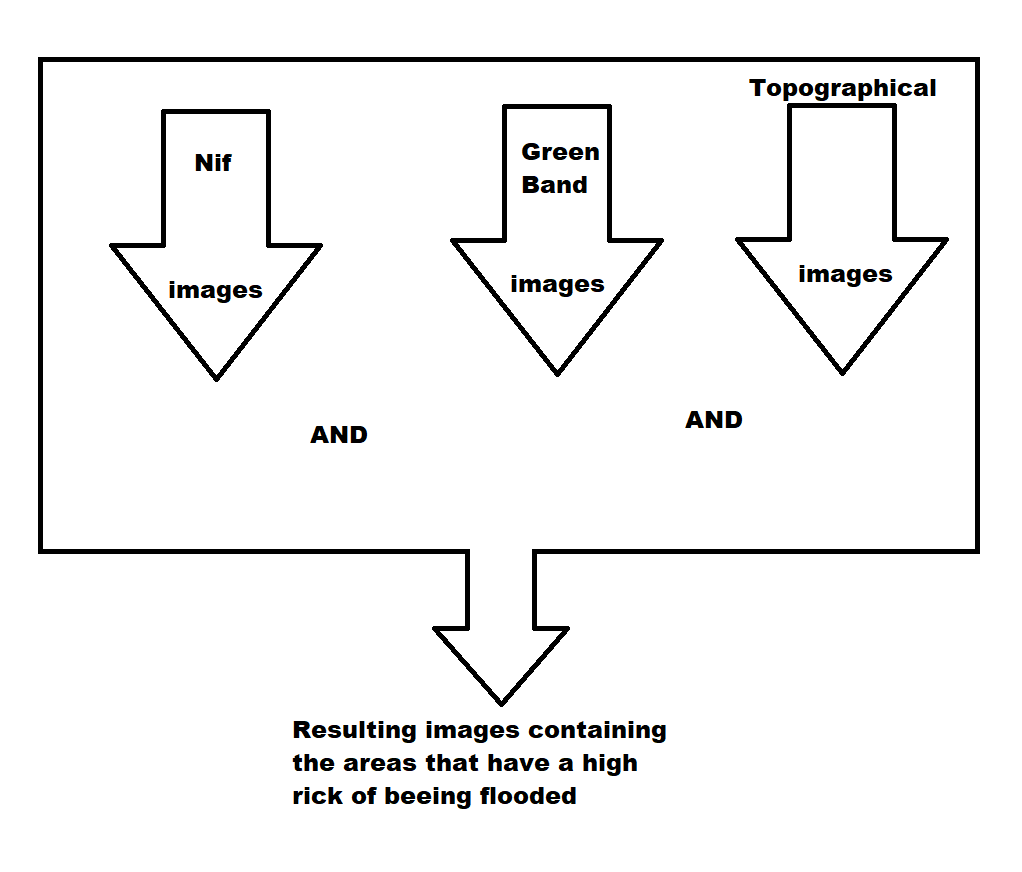
\includegraphics[scale=0.6]{application_outline.png} 
	Figure 1. Input and output description of the application.
\end{center}

Combining these techniques with an easy to use and understand client interface, we managed to create a system that can predict the land areas with a high potential of being flooded. The processing time and cost are reduced because the server has to go through a set of images only twice, first time to detect the surface water and second time to flood the land area based on the topographic map, so the computations are reduced as much as possible. From the user's point of view there are big advantages because the set of resources (satellite images) are free and easy to access and the results are easy to understand, making this application ideal for an untrained person.
\par





\subsection{State of Art of Physically models in flood prediction}

\quad
For creating our physical prediction model we chose to use NDWI water extraction technique due to the ease use and low processing time. McFeeters \cite{McFeeters} developed the normalized difference water index (NDWI) using the reflectance of the green (band 2) and near-infrared (band 4) bands of Landsat TM (Thematic Mapper). NDWI is one of the most widely used water indices for a variety of applications, including surface water mapping, land cover analyses \cite{Duan, Poulin, Hui} and it has also shown a great accuracy in classifying areas that include shadows and dark surfaces.
\par 

Besides the NDWI index for detecting the water bodies, there are some other techniques presented in various papers \cite{Multifractal water analysis, NDWI Comparison} that have shown significant results. These methods are the \textbf{Multifractal analysis of water bodies using Wavelet method and Fluctuation analysis} and the \textbf{detection of water using neural networks}. Both of these techniques have shown a high accuracy (multifractal analysis shown the best of those two, over 89\%; very similar to the accuracy obtained by the NDWI index).
\par 
There are some downsides regarding the neural network water detection. The method has shown great results but only on some particular sets of images and it did not provided a proper classification for all radar images. The studies \cite{NDWI Comparison} suggests that the neural network errors may appear due to the high sensitivity to noise in the images. 
\par 

In short, after our model manages to detect the water areas from a picture, it starts to expand these areas taking into account the topography of the land, like a flood bases to the land level. This model is called a physical prediction model and it allows us to create a simple to understand and test model, which will be time and cost efficient. 
\par 

There exist more complex physical models that can take into account more elements, like land water saturation, vegetation type of the area and the volume of rain that will fall over specific areas, but those types of models are more complex, and more expensive, both on execution time and development time. The test and validation part will need to be more complex, and the input required will be harder to obtain by a simple user. 
\par 

Besides the physical prediction models, there are some other forecasting models presented in various papers \cite{Flood forecasting models}, like data driven models based on machine learning and hybrid models that combine physical, and machine learning hydrological models.\par 

The first one that we will discuss is the \textbf{ML-based hydrology-dynamic modeling}: The computational cost of this model can limit the resolution and the scope of the hydro-dynamic system. The costs can be reduced by up to orders of magnitude by taking advantage of machine learning derivation methods, as it was experimentally done of other fluid dynamics models \cite{Yohai}.
\par 

The second model that we will discuss will be the \textbf{Remote discharge estimation}: The most important obstacle for incorporating machine learning into the hydrology field is the limited data. Measuring the water levels and the discharges is relatively difficult when taking into account the global order of 100,000. But even so the quantity, variety and quality of satellites constantly imaging all the rivers is rising at a very fast pace. The ability to estimate the river discharges without in-site measurements is a task that has become both critical for the hydrology field, and incredibly well suited for the field of machine learning.
\par 

The third and last model that we will discuss is the \textbf{Hybrid physics-machine learning hydrologic models}: This model is an alternative to the machine learning approach, and it adopts a hybrid approach where an ML model is combined with the classical physics-based components, which can enclose important prior knowledge about the domain structure. Some could view this approach as allowing the physically model to capture the major hydrologic  model, while the ML will be responsible for error correction, and calibration of the final model. An interesting fact is that it was shown that the physical models tend to be more accurate in the long-term and mid-term predictions, while the ML models tend to be more accurate in short-term predictions and, by combining those two techniques, it is possible to obtain an accurate prediction model on both long-term and short-time periods.
\par 

We chose to create a physical prediction model which combines the water detection technique (using NDWI index) with a flooding technique (based on expanding the water areas taking into account the topography of the land) because these approaches allowed us to create a simple model with a considerable accuracy rate (\textbf{67\%} calculated from our tests). With a less complex model we could save a lot from the developing cost because the required tests are much simpler to be done and the actual model is simpler to create, requiring less developers, less time and less money. Another good reason why we chose a simpler model is that its required processing time is reduced because it does not have to take in consideration as much factors as the ML or hybrid models. 
\par 

As a side effect of the reduced number of factors taken into consideration  by our model the consumer public has less gathering to do (gathering of information).


\newpage{}


\chapter{Problem description and solving}

\section{Technologies used}

\subsection{Collecting and processing the resources}

\subsubsection{Collecting the resources}

\quad
Our prediction model was created with a simple scope in mind, to offer a simple  application that can predict the areas with high risk of being flooded during a rainstorm, with as little processing time and cost as possible. The input for our model had to be easy to obtain and the output easy to understand, so we chose to use input data that is easy to obtain and free (it will need to be accessible by every person). The input for our model is a set of .tiff images that should contain a near infrared image (NIR), a green band image, and a topographic image. A simple way to obtain the NIR and green band images is by using the available data offered by satellites like Landsat 1 to Landsat 8 or Sentinel 2. 

\par 
The Landsat project is one of the longest-running enterprise projects for acquisition of satellite imagery of Earth. The project was first developed by NASA and then it was transferred to NOAA (National Oceanic and Atmospheric Administration) by U.S Jimmy Carter's presidential directive. There were 8 Landsat satellites on the Earth's orbit, now only 2 of them are still active, and the resources collected are available on the USGS (U.S Geological Survey) website. The only thing that a user will need in order to access the data is a free account. After the account is created the user can select different areas via USGS's EarthExplorer portal and download the satellite imagery using different filters.
\par

\bigskip

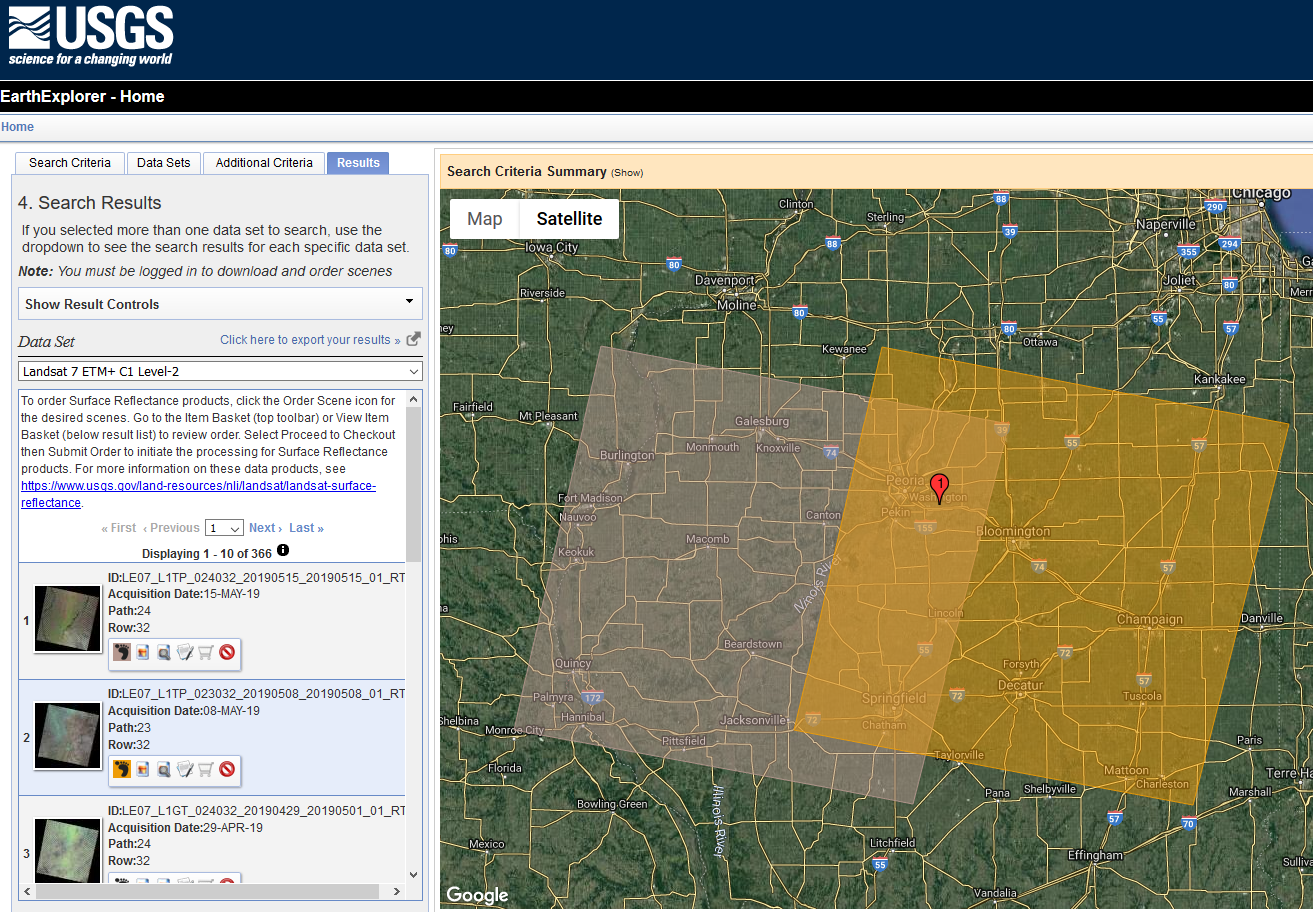
\includegraphics[scale=0.5, right]{landsat_search.png} 
\begin{center}
Figure 2. \cite{USGS} - Selecting Landsat images.
\end{center}


The image presented above (Figure 2) is a shot taken while searching for our test data from a region in U.S (Cairo) that was heavily flooded during a rainstorm by the Mississippi river. The yellow and pink areas represents two different scenes captured by the Landsat 7 satellite. A set of 8 images are found in a package downloaded from this website depending on the satellite that had provided them, but all of Landsat's satellites imagery sets contain a NIR and green band shot of the selected area (the main difference between them is the resolution in meters of the photo). In our research we mainly used Landsat's 7 images because the photos are at a higher resolution (30 m) and most of them are already processed by the USGS servers (some images need to be processed by the internal servers before being available to the users).

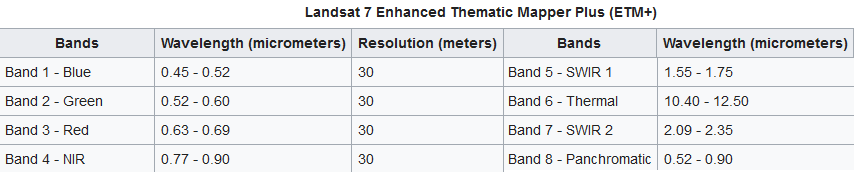
\includegraphics[scale=0.73, right]{Capture.png} 
\begin{center}
Figure 3. \cite{Wiki_landsat} - Landsat 7 bands description.
\end{center}


\medskip

As we specified above there are other options to obtain the images, besides Landsat, that is through the Sentinel program. Sentinel is an observation mission from the EU Copernicus Programme that acquires optical imagery of Earth at large resolution (10 to 60 m) over land and coastal waters. There are 3 satellites launched by the Copernicus Programme but we will focus mainly on Sentinel 2, because it has the largest collected data. 
\par 

The Sentinel 2 satellite has a multi-spectral instrument with 13 spectral channels in the visible, short wave and near infrared spectral range. The bands that are interesting for us are the 3-rd band which is the green one and the 8-th band which is the NIR one (the bands have a spatial resolution of 10 m). The images  can be downloaded from the Copernicus Scihub website, by creating a free account. There is a possibility to select a date range, cloud coverage percent and the satellite platform which is the best suited for the user needs (I.E Sentinel 1,2 or 3). 
\par 

There are some drawbacks regarding the Cepernicus Schihub website about the images accessibility. The site offers only two images that can be downloaded each day. The image preview will still be available, but none of the satellite image sets will be available for download. 
\par 

The website will display a map over Earth's surface and the user can select an area from where the images will be searched. Because the Sentinel satellites have a predefined trajectory some images can be a little bit cut of, meaning that even though we selected a specific area the images offered by the website can have some black parts representing the areas which the satellite didn't capture in the photos. We can see that thing in the left side of Figure 4, where a preview over the images is displayed.
\par 

A quick solution to this problem is to download adjacent images and merge them together into a bigger image using the tools offered by QGIS (we will discuss about QGIS in the following pages).

\newpage
\bigskip

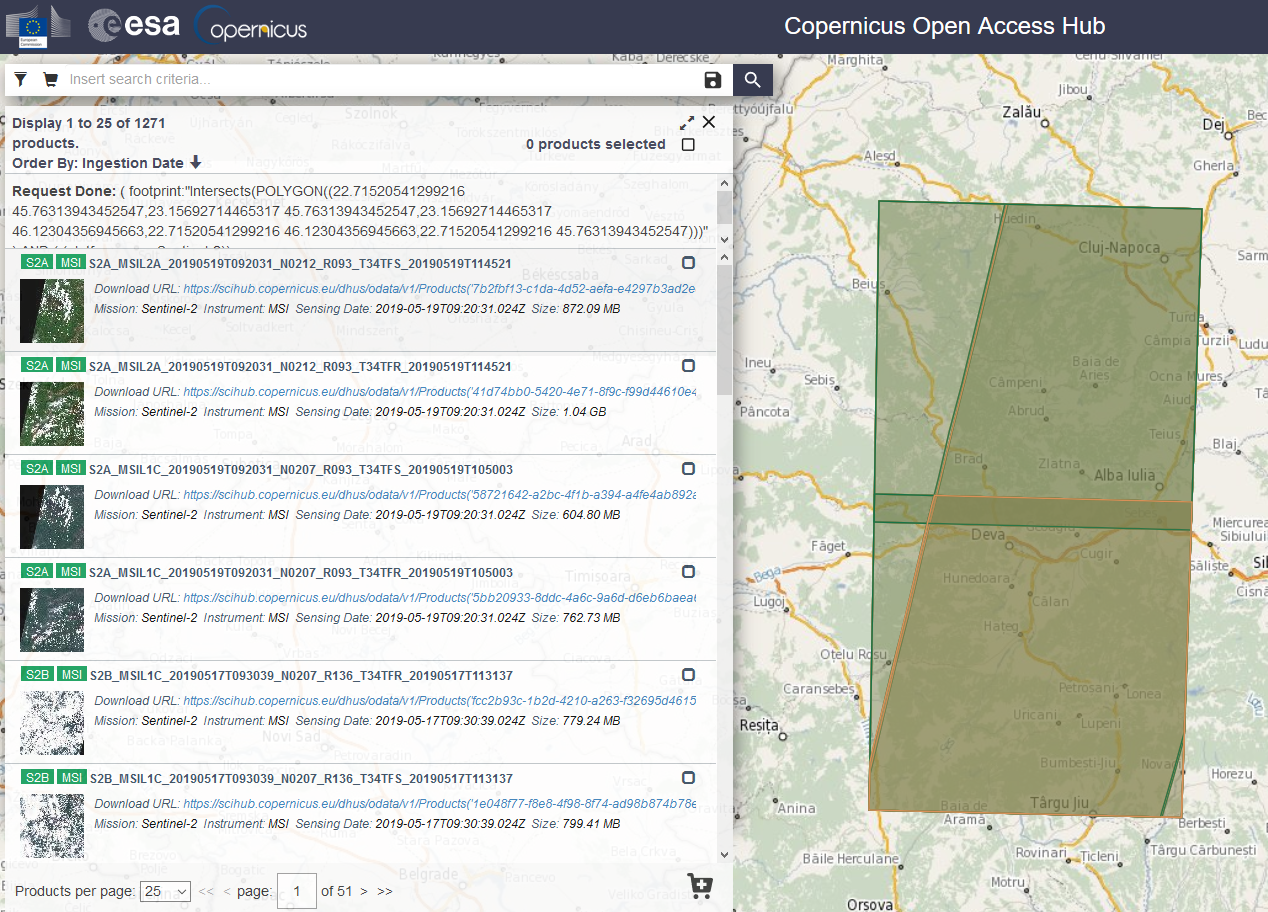
\includegraphics[scale=0.5, center]{sentinel.png} 
\begin{center}
Figure 4. \cite{Copernicus} - Selecting Sentinel images.
\end{center}
\par 


Still, there are some drawbacks from using the Sentinel imagery. We chose to use the Landsat images over Sentinel's data set because the Sentinel 1 images have a lower resolution, while the Sentinel 2 and 3 images are too recent (the satellites were launched in 2015, so the data set could not cover a larger time period for our analysis).
\par 

After we obtained the NIR and green band images we will need to download a topographic map of the area that will be processed. The topographic map can be taken from USGS website by searching for digital elevation maps. The process is pretty similar to the one of collecting Landsat imagery. An interesting difference between a NIR and a topographic image is represented by the image size. The topographic image is usually taken over a larger field, and this is a problem that we encountered during the processing of the areas with high flood risk. We had to determine where to place the smaller image inside the bigger one, based on global coordinates, but we will discuss this problem in one of the following sections.
\par

\subsubsection{Processing the resources}

\quad
Before a set of images can be processed by our application they need to be rendered. For this process we used a program called QGIS. Qgis is an open source geographic information system, created by OSGeo (Open Source Geospatial Foundation), licensed under GNU, that supports numerous vector, raster and database formats and functionalities \cite{QGIS}.
\par 

The images will need to be rendered from 8 bit depth to 32 bit depth and the pixel range value will be mapped between 0 and 255. They will also need to be saved with .TIF extension, to be later processed by our servers.
\par 

The Sentinel images are pretty straightforward to render, but the images from Landsat will need an extra step before being ready to save. The Landsat 7 images have what seem to be "black stripes" across the side of the image. This is due to a failure of Landsat 7 Scan Line Corrector. The forward movement of the satellite on the orbit should be compensated by The Scan Line Corrector, but because of the failure, a zigzag pattern for ground tracking is used instead of a mapping in straight lines. This can be seen very clearly in the image below (Figure 5), and the location of the black stripes varies between 390-450 m; therefore US Geological Survey(USGS) estimates that affected images lose about 22\% of their data \cite{Landsat-error}.

\bigskip

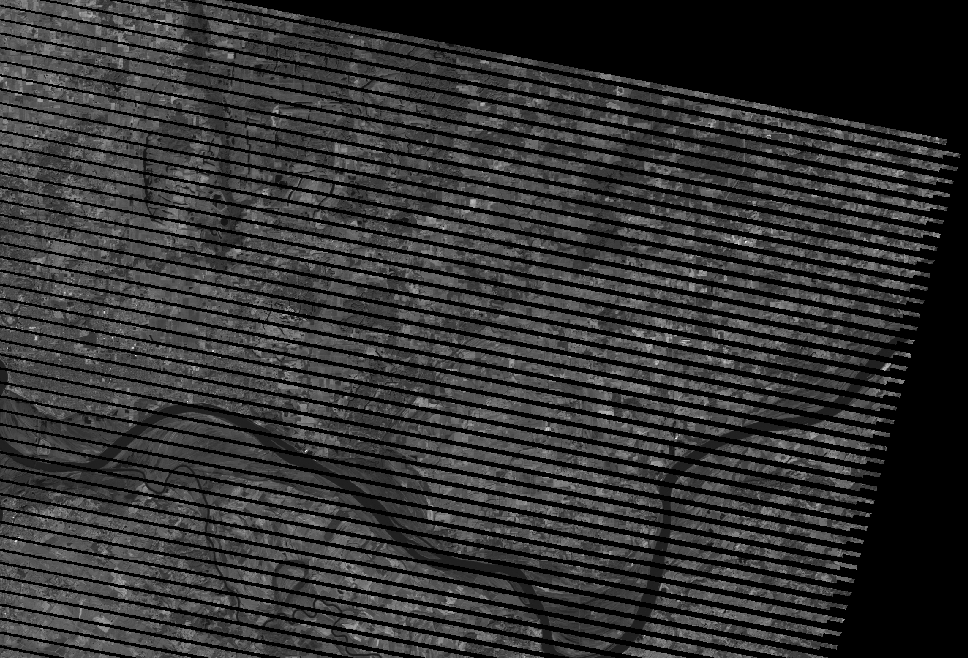
\includegraphics[scale=0.54, center]{landsat_black_stripes.png} 
\begin{center}
Figure 5. Landsat 7 image error.
\end{center}
\par 

\quad
The black lines get smaller as we approach the center of the image, which means that we can crop some parts of the land area and use them without any future modification, or if we need to use the full image we can try to apply an image correction, which should fill the black lines based on the gap masks offered by Landsat (for this part we will need to have Gdal installed). Below we can see how a mask layer looks like (Figure 6).
\par 


\bigskip


\includegraphics[scale=0.54, center]{landsat_black_stripes_correction.png} 
\begin{center}
Figure 6. Landsat 7 correction mask.
\end{center}
\par 

After the images are ready they can be rendered by saving the images with a .tif extension and checking the "render image" box.



\section{Programming languages and Frameworks} 

\subsection{Programming language: Java}
\medskip

\quad
Java is a popular object-oriented programming language that was designed to have as few implementation dependencies as possible. It was created in 1995 by Sun Microsystems and now it is owned by Oracle.
\par

This project was developed using Java 1.8 with two external libraries i.e.: Gdal and jai-imageio-core 1.4.0. Any version below 1.6 will now work as intended because of jai-imageio-core library. These libraries are used to process the TIFF images from satellite.
\par

At first we intended to use Python as the heavy lifting programming language because of the more relaxed syntactic structure, but in the end we chose Java because of its parallel programming capabilities. Usually when we have to work with satellite images we should take into account the fact that the images can be really large, around 8161x7211 pixels in size covering over 589.000.000 $km^2$, and when we have to process more than one image of this kind the processing time becomes very important.
\par

Python will become much slower in this area because of the Global Interpreter Lock or GIL (a mutex, or a lock, that allows only one thread to be in a state of execution at any point in time). The impact of the GIL is visible only to developers who execute multi-threaded programs, because it can create a performance bottleneck at the CPU level.
 \par
 
\bigskip

In the following image (Figure 7) we can take a look over the processing time (in milliseconds) between Java's multi-threaded system and the single-threaded Python system
\par

\bigskip


\par 
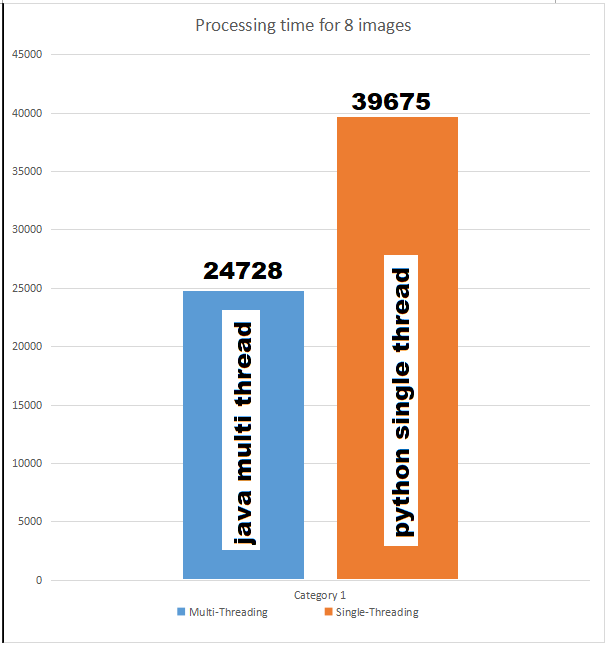
\includegraphics[scale=0.7, center]{multi_thread2.png}
\begin{center}
Figure 7. Java multi-thread vs python single-thread; time milliseconds.
\end{center}

\quad
The tests were made by us on a sample of 8 images with an average size of 1000x1000 pixels, and the result have shown that the java multi-threaded system (marked with blue on Figure 7) was in average 40\% faster than the python single-threaded system. We value this feature very much because the reduced processing time combined with the image handling power offered by java helped us to create a time and cost efficient application.


\subsection{Programming language: Python}
\medskip

\quad
Python is an interpreted, high-level, open source programming language that was made to have a relaxed syntactic structure and to be more easy to read. It supports both functional and object oriented programming and its mainly targeted to a fast development and easy to maintain code.
\par

Python has played a major role in the project because of its relaxed syntactic structure and it was used to create the server part of the application, using Flask (flask is a microframework for python web based applications).
\par 

After the server receives a set of satellite images from the user, a Java process is started by the server to solve the request. The java files are complied when the server is started for the first time, and then for every incoming request a java process is started. All this part was handled using Python's "subprocess" library
\par
\medskip

We will take a look on how the python server compiles the java files and how a process is started, and we will discuss in more detail in the following chapters.
\medskip

Here we can take a look on how the java files are compiled
\par
\bigskip
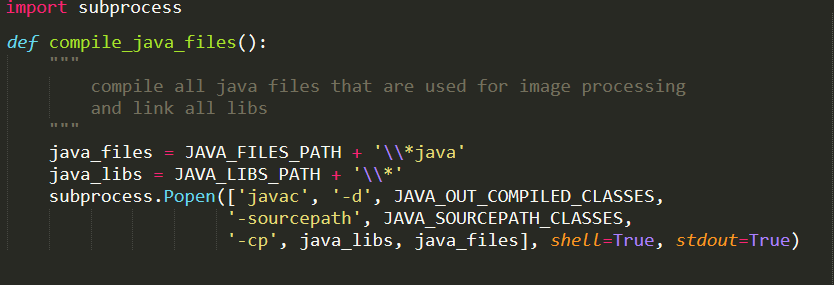
\includegraphics[scale=0.8, center]{python_call_java_1.png}
\begin{center}
Figure 8. Compiling Java files on python server.
\end{center}

\newpage

Here we can take a look on how a process is started
\par
\medskip
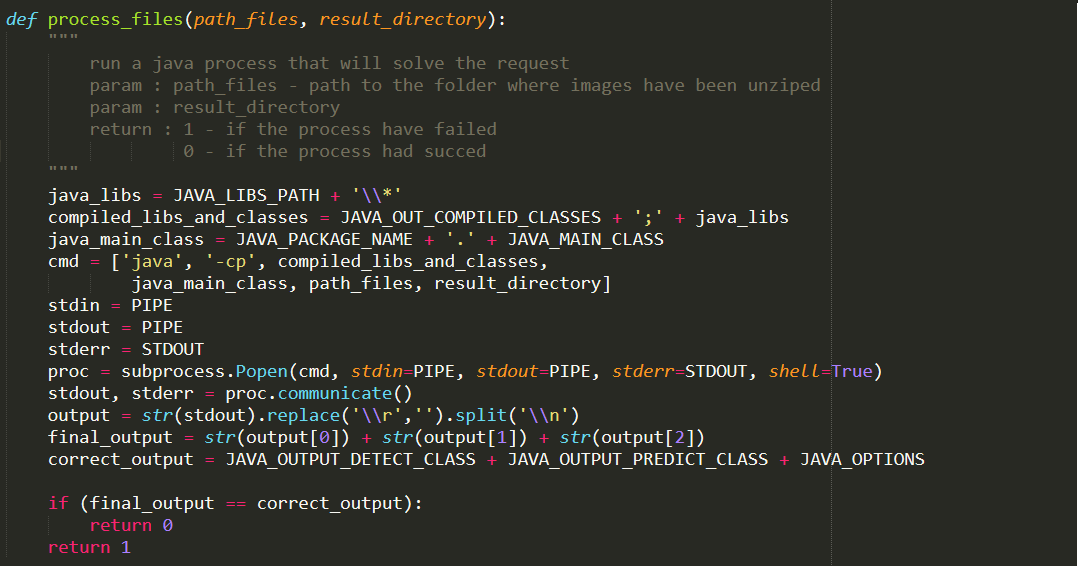
\includegraphics[scale=0.7, center]{python_call_java_2.png}
\begin{center}
Figure 9. Spawn a Java process from python server.
\end{center}

\subsection{Gdal Library}

\quad
Gdal (Geospatial Data Abstraction Library) is a software library available for multiple programming languages (python, java, c++) for manipulating rasters and geospatial data vectors. It was released by the Open Source Geospatial Foundation (OSGeo) in the year 2000 with a permissive X/MIT free software license\cite{Gdal}. 
\par 

We used Gdal as a Java library to process the satellite images. We needed a way to extract the coordinates of specific pixels from .Tif images, and The Gdal library offered a convenient way of doing that by using gdal.Datasets, gdal.Band and the GeoTransform matrix.

\subsection{Flask Framework}

\quad
Flask is a web framework written for Python which is classified as a microframework because it does not require particular tools or libraries. It's considered a lightweight framework because it has no database abstraction, no user authentication and no form validation.
\par 

Flask was developed based on the template engines offered by Jinja 2, which enable an accelerated development for our web application. It also offers a micro, but extensible, web framework, which can become very flexible by using several widely used web development tools and libraries \cite{Flask1}.
\par 

There is an another available web framework dedicated to Python which we took into consideration when we built this application namely Django. At first look, Django seemed a better choice than Flask because it has a better template engine than Flask, it has an ORM (object-relational mapping) system that can work with several databases like SQLite, Oracle and MySQL and it has a built-in bootstrapping tool, but despite all these upsides which can make the application development much easier, there are some drawbacks when using Django. Even though Django could offer a cheaper application development, we should also take a look on how a Django HTTP server will compare to an HTTP Flask server.
\par 

We had to consider the fact that the machine on which our application will run will need to be cheap to maintain and responsive, which means that it should have low latency (that was one of our main focuses). We have taken a look on several benchmarks that compared the performance obtained by Flask and Dajngo during longer sessions of run time. The available resources tend to change with time so we need to be cautious. We had to determine how they can handle a more intensive environment where the available resources can decrease. Like on real machines where the decrease of resources is non-linear, because the OS can spawn daemons or trigger some side jobs, we had to find some tests that will take these facts into account. In these conditions we found that the HTTP Flask server performs much better than the HTTP Django server. The tests that we have taken into consideration \cite{Flask2} were made using Gunicorn (a Python Web Server Gateway HTTP interface) at a constant rate of 4000 queries per seconds. In the tests the HTTP Flask server displayed lower latency and error numbers and a higher request number compared to the HTTP Django server.
\par 

\medskip
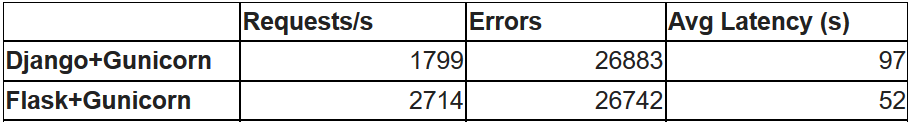
\includegraphics[scale=0.6, center]{django-flask-table.png}
\begin{center}
Figure 10. \cite{Flask2} - Table Django vs Flask.
\end{center}

\medskip
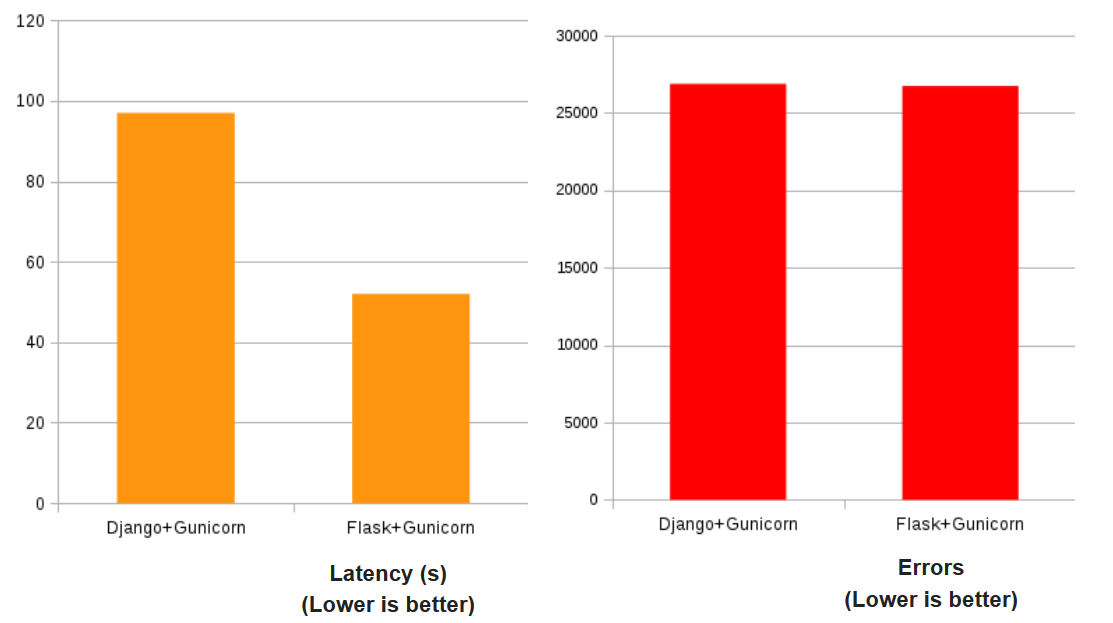
\includegraphics[scale=0.6, center]{django-flask-latency.png}
\begin{center}
Figure 11. \cite{Flask2} - Latency and error diagram (Flask vs Django).
\end{center}




\section{Functional description}

\quad
In this section we will take a closer look on how our application manages to process the input offered by the user and predict the areas with high flooding risk. Firstly we offer a friendly and easy to understand web interface where any user can upload a set of satellite images. A set is composed of a NIR image, a green band image and a topographical image.
 After the input is uploaded to the server a solving request will be created and placed on a queue. Each request is processed one at a time and when its turn will come, the server will unzip the input and start the prediction. The first step in our prediction consists in detecting the water surfaces by combining the NIR band image and the green band image, then applying a formula called NDWI (Normalized Difference Water Index) to each pixel. After that, the resulting image is mapped to the topographical image and a flood algorithm is applied. The flood will start from the water bodies already detected and it will spread based on the land's topography.

\newpage
\subsection{Detecting surface water using NDWI}
\quad 

The detection of the water bodies was probably one of the most challenging part of this application, because there are different types of water, with different colors and different densities. At first, we tried to detect the water surfaces based on their color, but usually the chromatic of the oceanic water is very different compared to the chromatic of the lakes and rivers. The color range that we had to cover was too large, so we gave up on this idea. 
\par 
The second approach was to use only the near infrared band. The idea behind this was that the satellite will shoot a laser beam across the land area and the beam will be reflected back by most of the objects, except for water. It is one of the only things that can absorb the NIR laser, so the values of the NIR resulting images over the water bodies will be equal to 0. Near the water banks, because the volume of water is too small to absorb all the NIR rays, the pixel values will not be exactly 0 (the value range can vary up to 15-20). The method seemed to work when we considered all the pixel values between 0-15 to be a water part, with a calculated accuracy of around 83\% (from our tests done over a set of 12 images), but we encountered a big drawback. On the flatter land areas, lacking valleys and mountains, the images looked pretty good, but when the topography started being to be a bit more diverse the shadows began to appear. The pixel value of the areas covered by shadows can vary between 10 and 25, so we got a lot of false positive cases.

\bigskip
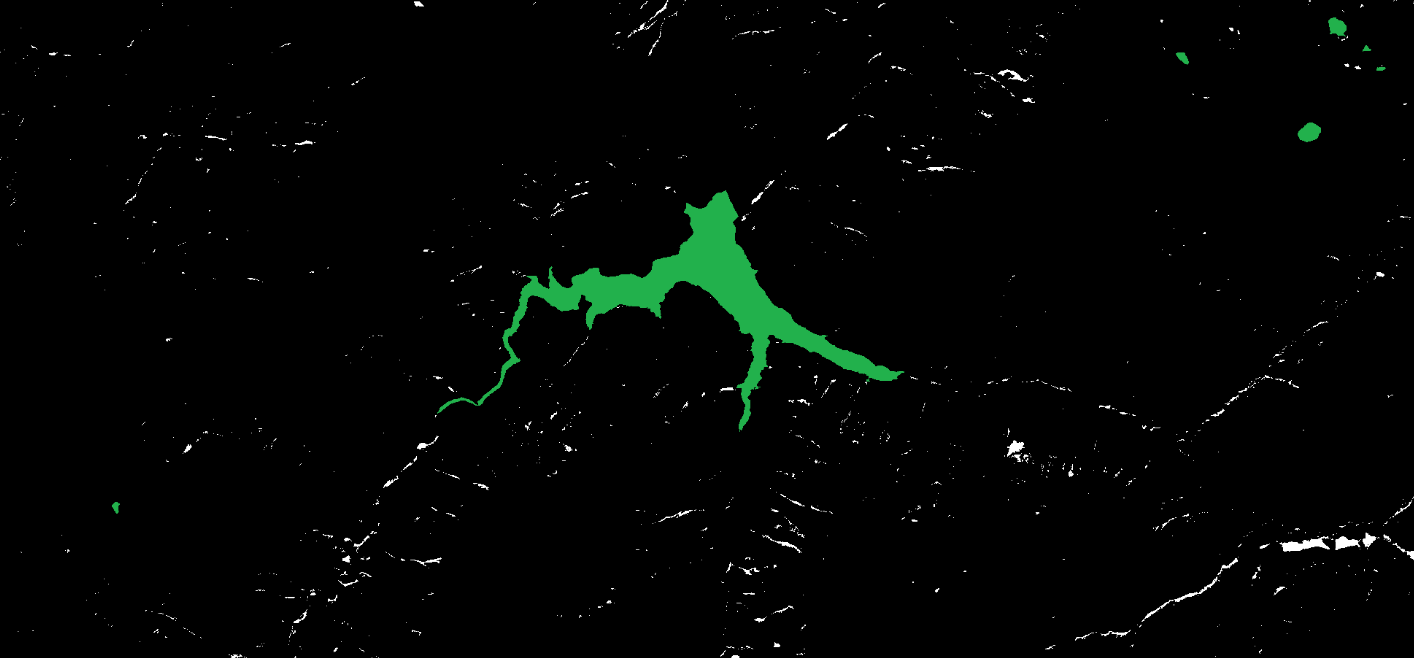
\includegraphics[scale=0.4, left]{water-false-positive.png}
\begin{center}
Figure 12. False positive water detection.
\end{center}
\par 

We can take a look at the previous picture (Figure 12) to see how significant the errors caused by the shadows are. The green areas represent the water bodies classified correctly and the white areas are the shadows that our application classified as water. It may not seem much but that figure is 1414 x 658 pixels in size covering around 930.412 $m^2$, and it will be a waste of money to move all the people from that area in case of a flood just because we classified the shadows as water.
\par 

The approach that we chose in the end was to use an index called NDWI or Normalized difference water index. NDWI is a remote sensing indicator which is obtained by combining the NIR and green band images. The formula will be applied as following for each pixel (Xgreen - color of a pixel from the green band image; Xnir - color of a pixel from the NIR image):

$$ NDWI/perpixel = \frac{Xgreen - Xnir}{Xgreen + Xnir}$$

If the calculated value is bigger than 0.45 we can classify that specific pixel as a spot that contains water, and all the other values below that can be classified as non-water pixels (land). This method has shown a very satisfying result compared to the true value, with a calculated accuracy of around 88\% (the tests were done by us over a set of 12 images; over the oceanic area the accuracy was around 98\% and over the more diverse land area the accuracy was around 82\%). The big advantage of this approach was that it does not identify any shadows as water pixels, without losing accuracy. 
\par 
There are numerous studies \cite{NDWI, NDWI Comparison} that suggested that NDWI is one of the best classification method, for optical images, comparable with the multifractal formalism method (with an accuracy of 89\%), and the neural network classification approach that shown great results in some cases, but it did not provide a proper classification because of its high sensitivity to speckle noise.
\par 

In the end, using this approach we manages to detect all the water bodies with a great accuracy with an insignificant false positive rate caused by shadows and other objects. We can take a look in the following picture (Figure 13) on how a result image using NDWI would look like. In this picture all the white zones are water areas, and if we compare Figure 12 and Figure 13 we can see a big improvement when we take in consideration the error caused by the shadows.
\par 


\bigskip
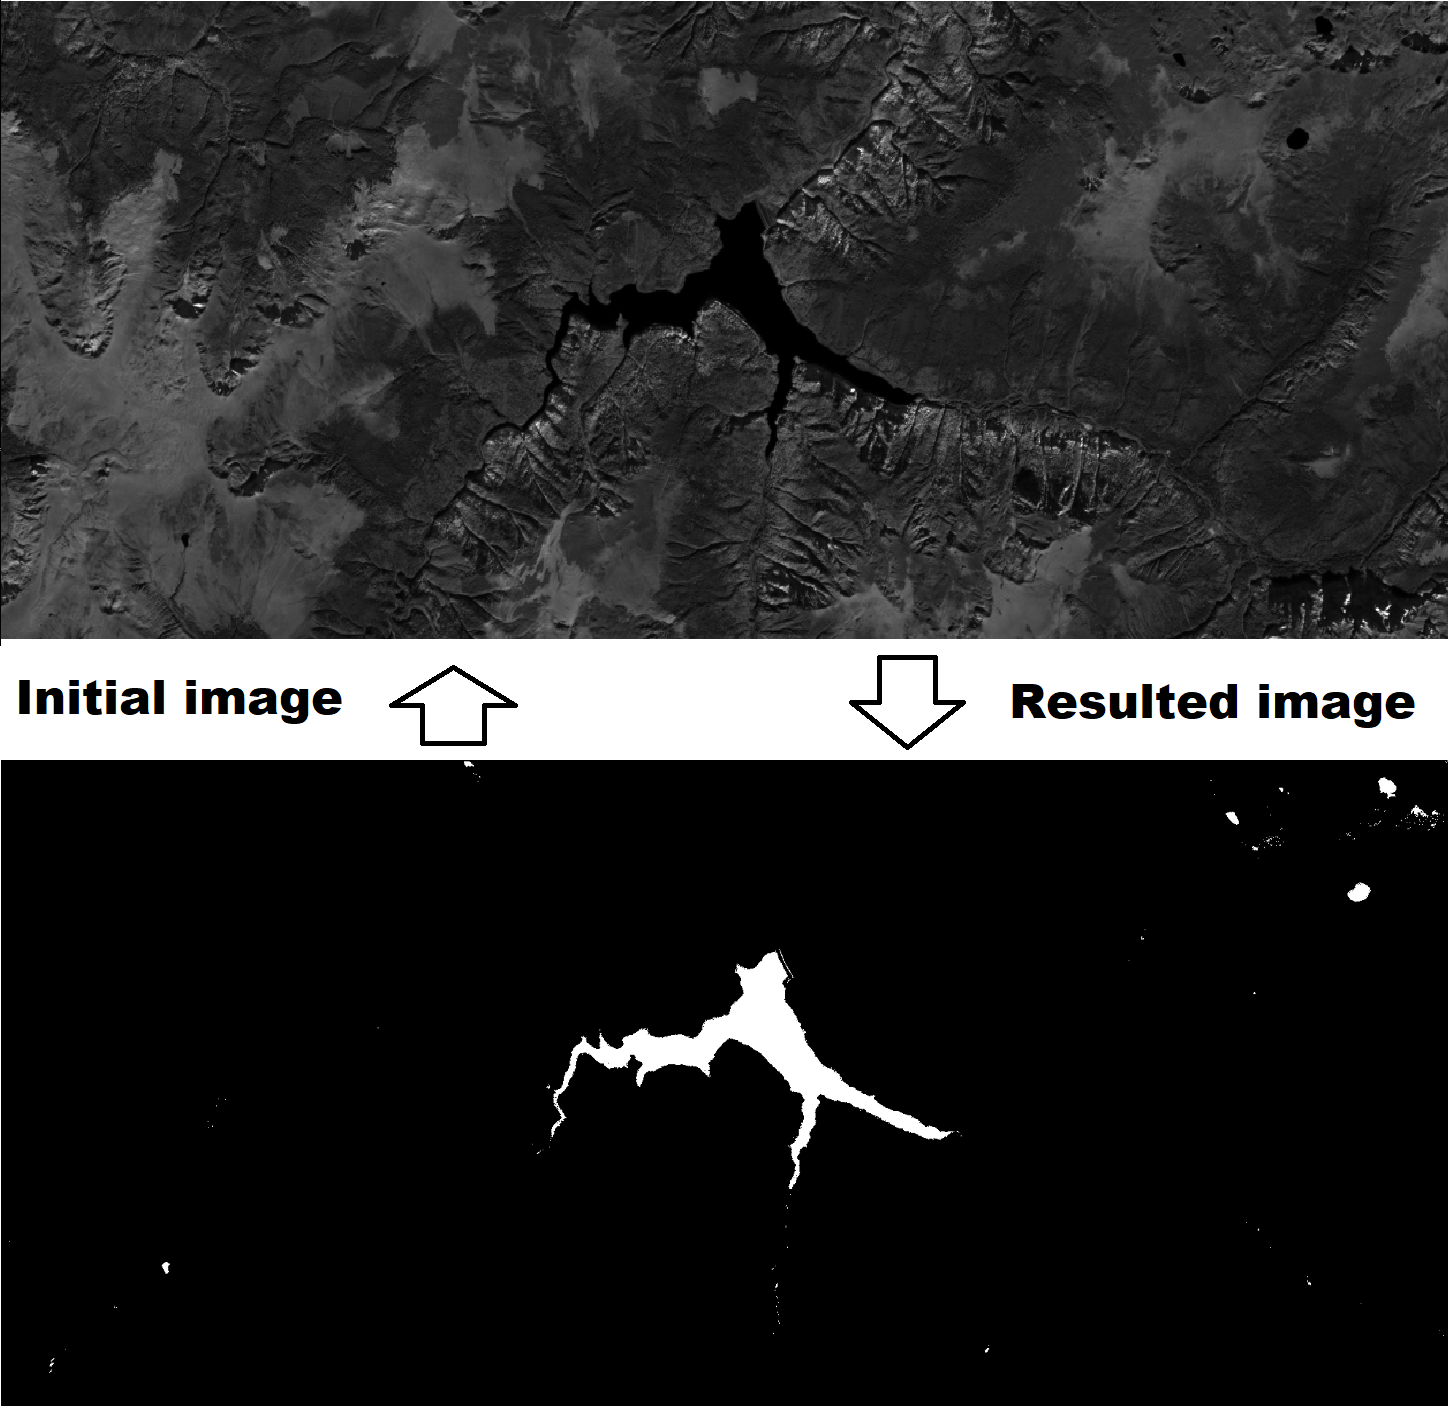
\includegraphics[scale=0.4, left]{NDWI-prediction.png}
\begin{center}
Figure 13. Water detection using NDWI (white areas are water bodies).
\end{center}
\par 

After the application has managed to detect all the water bodies from an image it will need to overlay the processed image over the topographic image. This will be a topic that we will cover in the next subsection.

\subsection{Mapping the processed images (containing water) to the topographically images}

\quad
In this section we will discuss about how we managed to map two images (the processed image, containing water, with the topographical image). The idea behind this process is that, usually the topographical images, available online, tend to cover a very large area, that can be even 10 times bigger than the image used to detect the water bodies, so when we apply the flood algorithm that should spread the water based on the topographical surface we cannot simply place the smaller image over the larger one without taking into account the coordinates. 
\par 

Fortunately for us, every topographical, NIR, and green band image offered both by Landsat and Sentinel has a header that contains the metadata (information about the data; structural, administrative and descriptive). In the header we can find the coordinates of each corner of an image, and we can use the Gdal library to take use of that data. The Gdal library can parse every header offered by satellite images and this is why we chose to include this library into our application. 
\par 

We cannot just simply overlay one image above another because the pictures can have different resolutions, some of them have a resolution of 10 $m^2$ per pixel, while others can have a resolution 30 $m^2$ per pixel. What we did instead was to create a function that can map every pixel to a global coordinate (of form longitude and latitude), which enabled us to search for that coordinate set in the second image. For every image header we apply a function offered by Gdal called dataset.GetGeoTransform, which can parse the metadata and then, based on obtained data, a Spatial Reference is created for each picture (Spatial reference is a class offered by Gdal that can reference every satellite image to a place on Earth based on the metadata obtained). The Spatial Reference for both images (our processed image and topographical image) is then passed as an argument together with the transformation header and the pixel coordinates to a function that will return the longitude and latitude corresponding to the specified pixel.

\bigskip
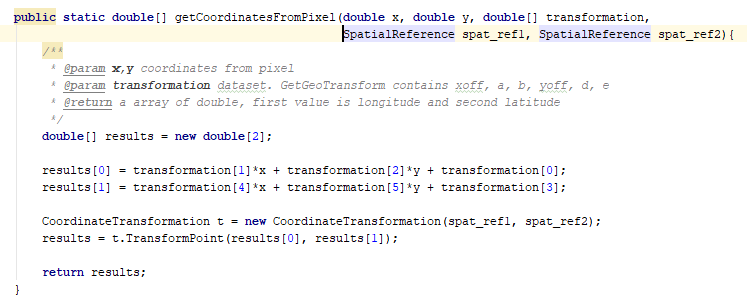
\includegraphics[scale=0.8, left]{java_coordinate_mapping.png}
\begin{center}
Figure 14. Function for obtaining global coordinates from pixel coordinates.
\end{center}
\par 

\quad
There is an another function created by us that can take as an argument the longitude, latitude, transformation dataset and the Spatial References for two images and it can return the pixel coordinates corresponding to the specified global coordinates.
\par 
These functions will be used to help us on the flood algorithm that we will discuss about in the next subsection.




\subsection{The flood algorithm applied over the images}

\quad
In this subsection we will discuss about how the flood algorithm works. Firstly the water detection class is called, which will combine the NIR and the green band images resulting in a processed image that will color all the water bodies with the white color while the rest (land cover) will be colored black.
\par 
 After the water is detected, the flood algorithm is called. The algorithm is stored in a class that will take as input parameters the name of the NIR image, the name of the processed image(containing the water bodies), and the name of the topographic image. The only reason that we had to pass as an input parameter the name of the NIR image is because our processed image does not contain a file header (containing the global coordinates of each corner), but essentially the images are pretty much the same, when it comes to the land covered area, so we had to use the NIR header as matadata for our processed picture.
\par

The flood algorithm that we created is based on the \textbf{square flood fill algorithm}. The idea is that the image is parsed in a linear manner, and when it encounters a white pixel (containing water) it starts a fill algorithm. That pixel will be colored to green and its height from the topographical map will be retained (the height is obtained by mapping the pixel from our processed image to the topographical map, using the functions described in the previous subsection). Every neighbor (up, down, left, right; this is why it is called the square flood fill) of that pixel will be place on a stack. \par 
The elements are popped from the stack, one at a time, and every element is checked. If the element is a white pixel (already containing water), it is colored green (we chose to color the already parsed pixels with green to know that they have been checked, so they will not be added again on the stack; it servers as a mark flag) and its neighbors will be added to the stack. If the element is a black pixel (land area) it will be subjected to a test, and if the test is passed the pixel is colored green, and all his neighbor will be pushed on the stack. 
\par 
The test consists on several things. Firstly the coordinates (set x,y) of the black pixel will be gathered from our processed image. The x,y coordinates will be transformed to a global longitude and latitude. The obtained global coordinates will be mapped to the topographical image such that the algorithm will be able to identify the exact position of our black pixel on the topographical map. The height of our black pixel is then compared to the previous stored height, and if the height difference is small enough, the pixel will pass the test. Beside the height difference we tried to take into account the distance from the river, such that we store the coordinates of the closest river (water) pixel, and calculate the height difference based on the distance from the water. The reason why we used this extra test was because of the swampy regions. These regions tend to be pretty flat, with a small height variation, but we all know that water cannot extend to infinity, so this is why we chose to use this extra case. The height difference that we accepted was between \textbf{$CurrentHeight - 2$} and \textbf{$CurrentHeight + 2$} (the range was selected by us based on several tests and comparisons with real floods).
\par 
In the following pictures (Figure 15, Figure 16) we can take a look on how our application will get through every process (detecting water and applying the flood algorithm). On Figure 15 in the left side we can see how a NIR input image would look like and in the right side is the resulting image after we apply the detection of water bodies.

\bigskip
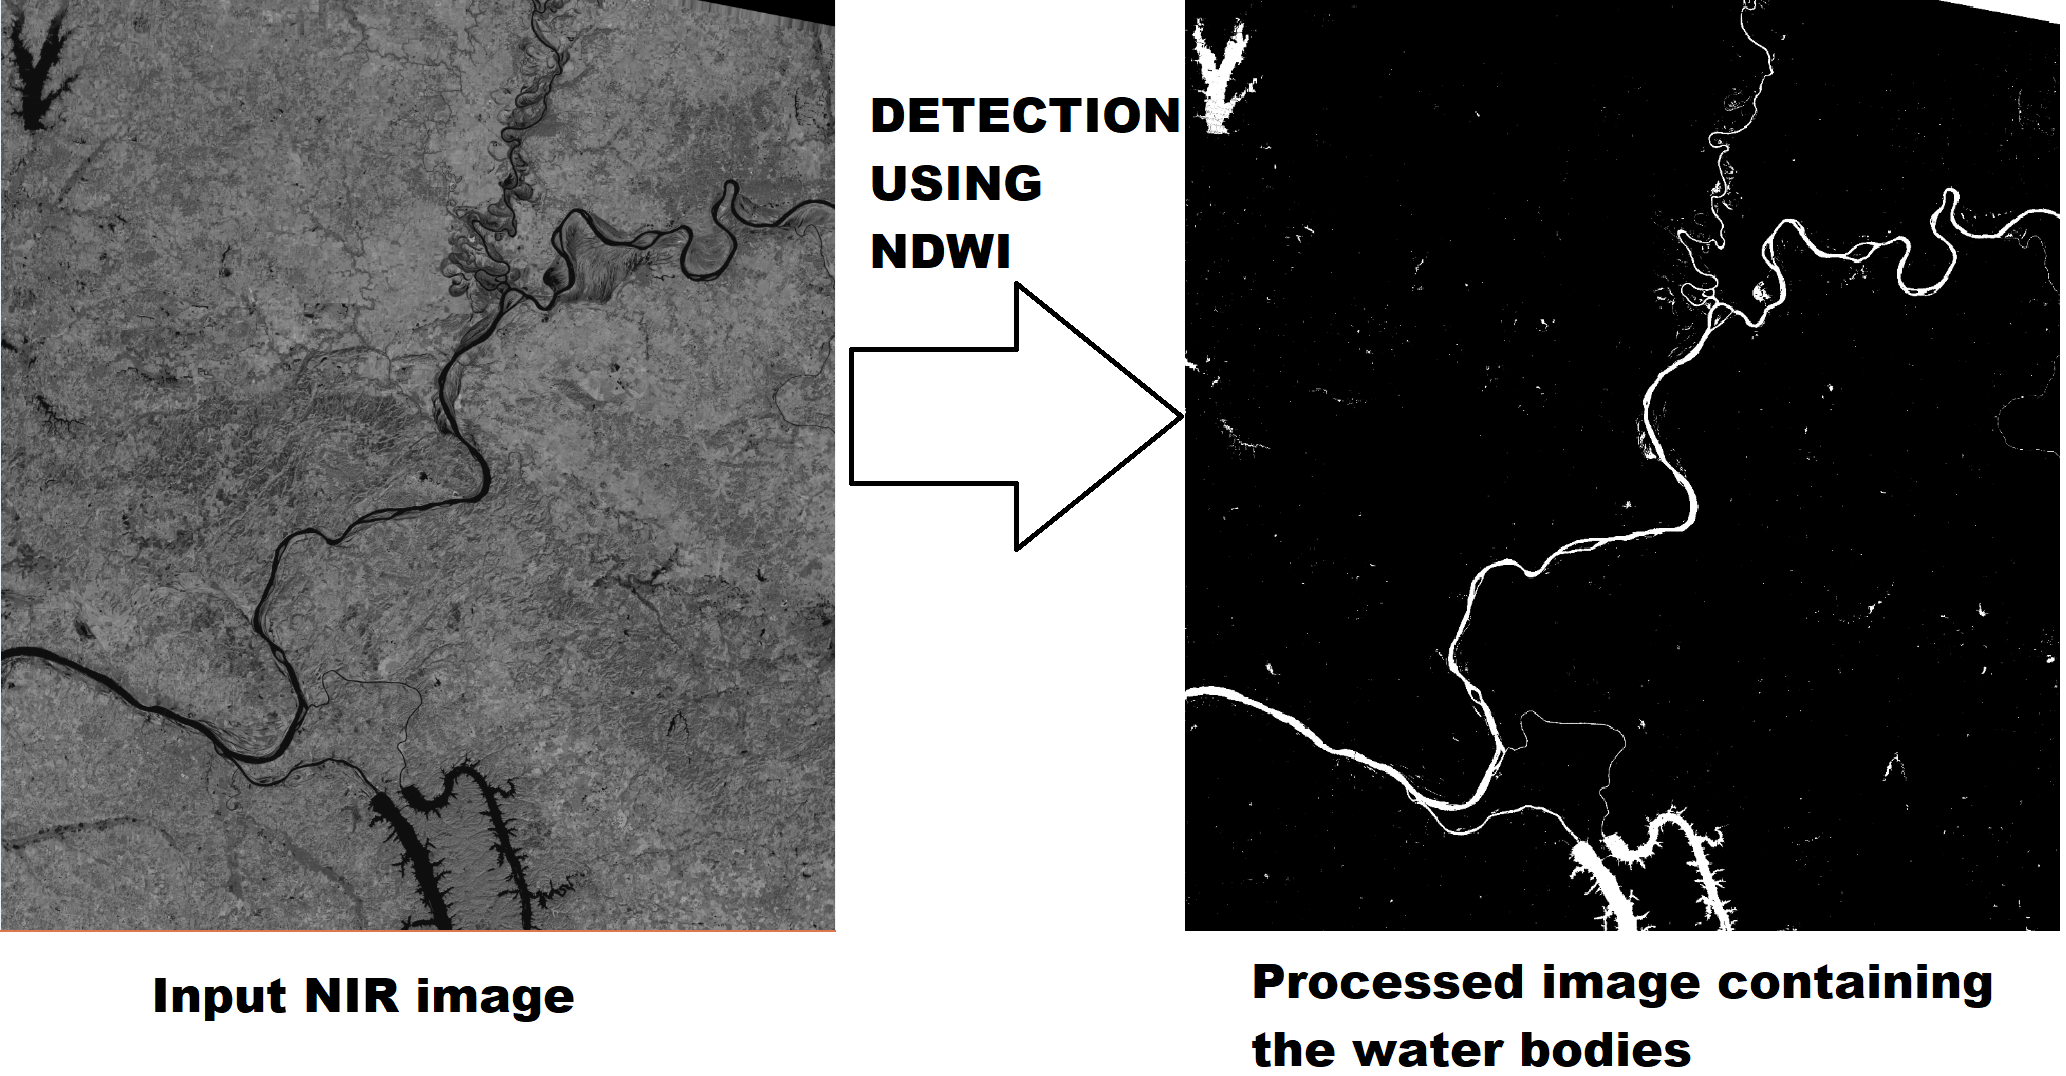
\includegraphics[scale=0.3, left]{process1.png}
\begin{center}
Figure 15. Detecting water bodies.
\end{center}
\par 

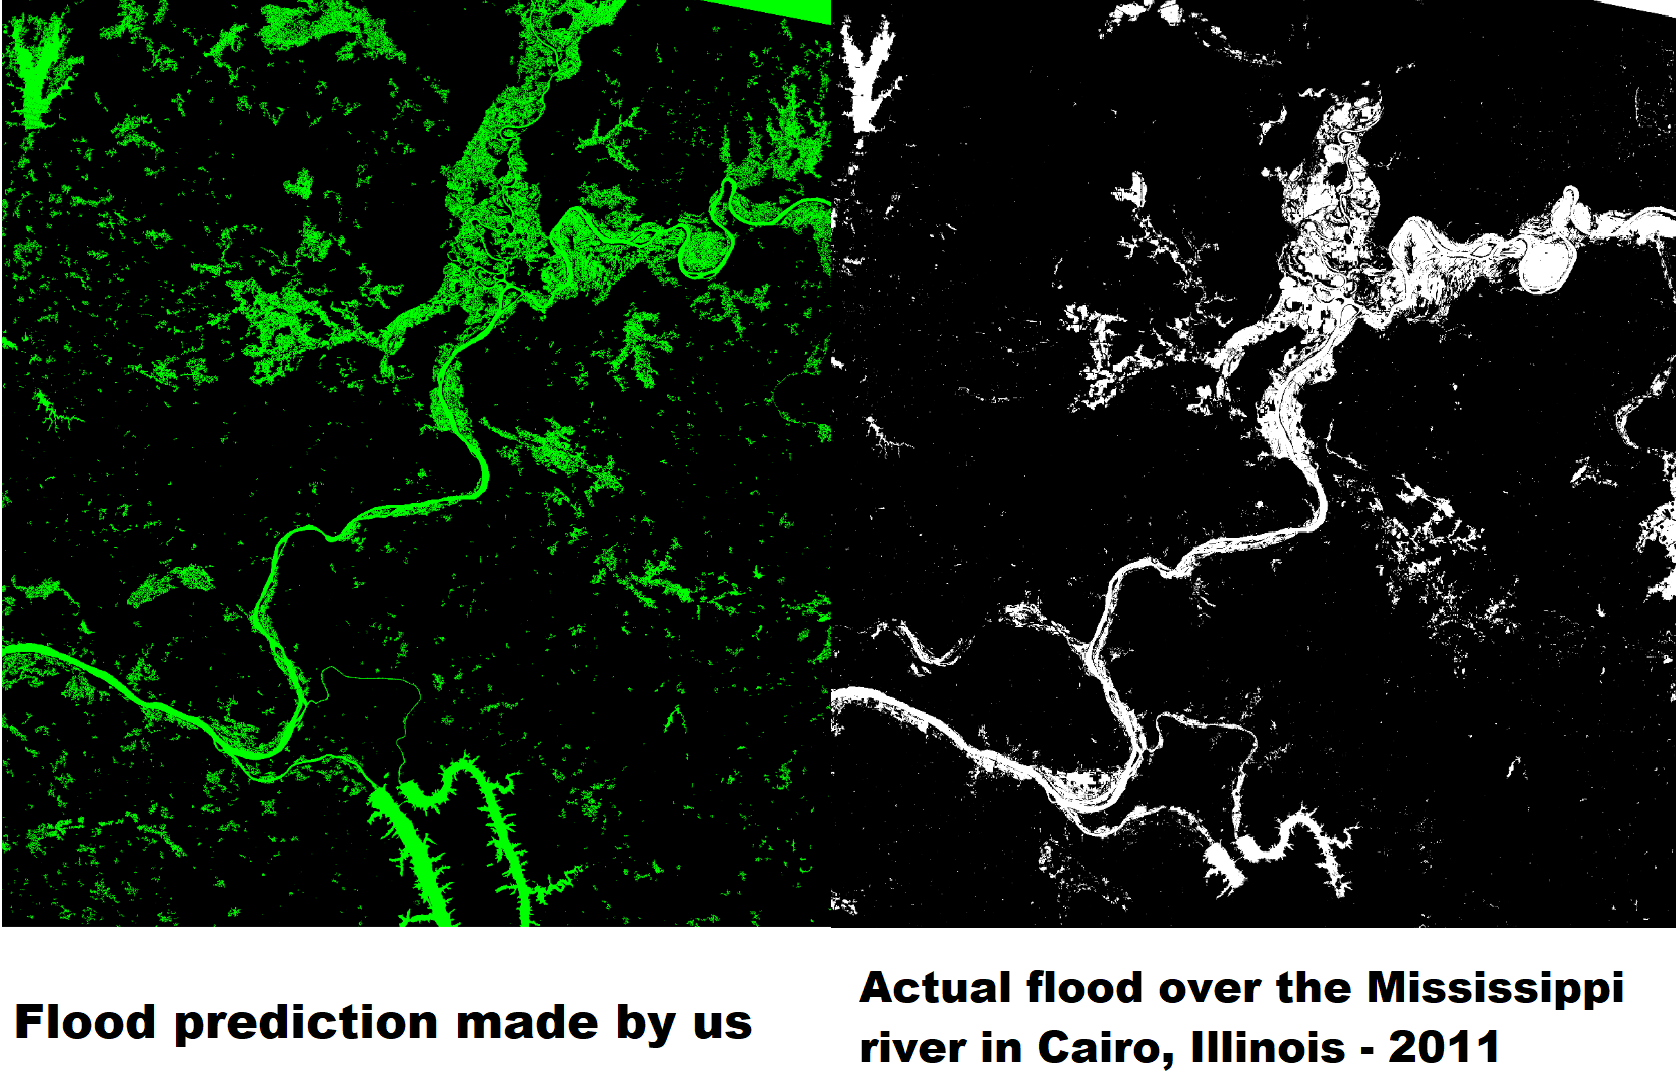
\includegraphics[scale=0.4, center]{process3.png}
\begin{center}
Figure 16. Our prediction and an actual flood.
\end{center}
\par 

In the above picture (Figure 16) we can see, on the left side, how a prediction made by our algorithm would look like. The image is obtained by applying the flood algorithm over the processed image (which contains the water bodies) on the right of Figure 15. \par 

On the right side of Figure 16 we can see an image of an actual flood area that was captured by the Landsat 7 satellite over a section of Mississippi river in Cairo, Illinois, USA. There are some zones  that contain water (in the image of the actual flood) that cannot be seen because of the clouds. The green waves cannot penetrate through the clouds, meaning that some images cannot be processed correctly because of this problem.
\par 

Another possible cause that can make some differences, between the two images, is the fact that our flood algorithm does not take into account the volume of water dropped over a specific area during a rainstorm. That kind of data can be hard to acquire by a normal user and can make the whole process much expensive, both on processing time and on application developing time. This is a thing that we take into account when we built the system, such that we can keep the whole application at a low cost. In the next figure (Figure 17) we will overlay the prediction made by us with the real flood and check the numbers.
\medskip
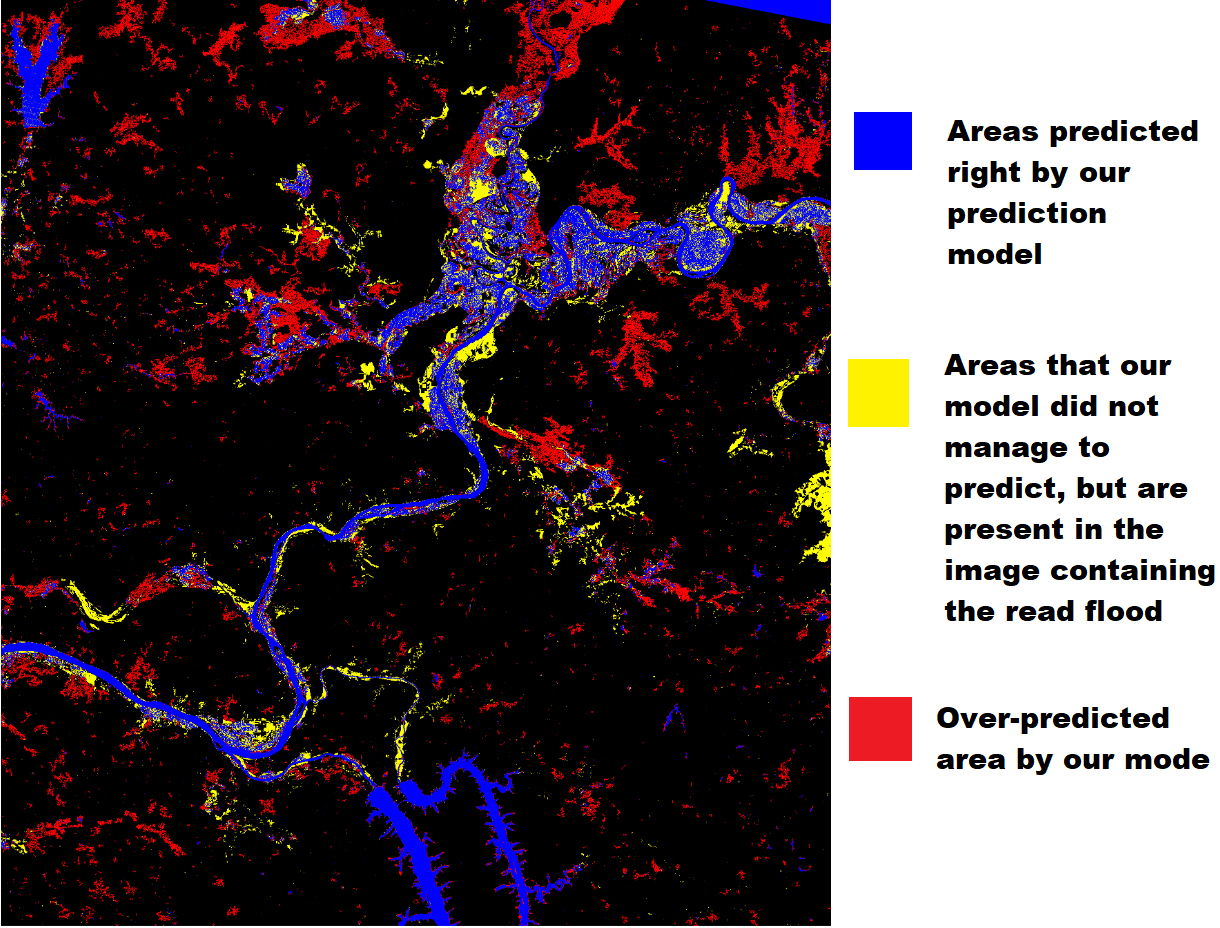
\includegraphics[scale=0.6, center]{processed_flood_combined.png}
\begin{center}
Figure 17. Our prediction compared with real flood.
\end{center}
\par 

The image above covers about 260,000,000 $m^2$ and it represents the overlaid images of the prediction made by us and a real flood that took place in 2011. The blue marked areas  represents the areas that our model predicted right which are \textbf{15,379,190} $m^2$ and the yellow pixels represents the area which was flooded in 2011, but our model could not predict. The yellow surface is about \textbf{7,801,780} $m^2$ in size, which means that our model has managed to predict the flooded areas with an \textbf{accuracy of 66,34}\%. The red pixels in the image represent the land area that our model overestimated, but we cannot classify that as an error because our prediction model does not take into account the precipitation level that will fall during a specific rainstorm, it just predicts the worst possible case. That red area covers around 8,976,000 $m^2$.


\newpage
\chapter{The application}

\section{Functional description}

\quad 
In this section we will describe how our application is structured and the technical details about the implementation will be presented in one of the following chapters called Implementation details. 
\par 

Firstly our application has a server side which is written in Python, using the Flask web framework, and that part will run as a process on our machines. It will offer a web GUI interface for every user that will choose to access our website. There are several HTML templates that will be loaded when needed (home page, image upload succeeded page, image upload failed page, error while processing page). 
\par 

The first page that is displayed when a user will access the website will be the homepage. On it the instructions on how to use our application will be displayed together with an upload files field (that would take a zip, tar.gz or taz.bz2 as input), and a field where the user can enter an email. On the upload files field the user can place as input a set of images. The sets should be composed as follows: one NIR image, one green band image, and one topographical image over the same are. The images should have the .TIF extension. The user can place multiple sets of images but the sets would be differentiated by their name (e.g set 1: \texttt{0\_nif}, \texttt{0\_green}, \texttt{0\_topo}; set 2: \texttt{1\_nif}, \texttt{1\_green}, \texttt{1\_topo}). The email is required because after the images are being processed the server will fire an email to the specified address with a link from where the resulted images can be downloaded.
\par 

After the submit button is pressed, the input images will be uploaded to the server; if the upload has succeeded and the email is valid an HTML page with that specific message will be displayed. When the images are received by the server a request to process the input sets is created and placed on a queue, each request is processed one at a time. A request will contain a field with the user email address and a field containing the path to the zip files that the user had uploaded.
\par 

When the time has come for a request to be processed, it will be popped from the queue and analyzed. The server will try to unzip the input set and check if the resulted folder contains the required images with the specified naming style. If the standards are not met an email is fired to notify the user that the input is not valid and it will not be processed. If the input set is accepted, the server will add in the Databese an item that will contain a path to the folder where the images were unzipped and a unique hash that should make the identification much more easy. The image processing part is done by a Java process that will be spawned by the server for each request. The Java files, together with the needed libraries will be compiled when the server is started for the first time (we already talked about how we compiled the Java files and how we run a Java process from python in the second chapter on python subsection; Figure 8 - compiling, Figure 9 - running a process). 
\par 

When a Java process is started the server will pass as command line arguments a path to the folder where the images that should be handled are stored, and a path to a folder where the resulted picture should be placed (the folder that will contain the results is created by the server). From this point the spawned Java process will handle the given input in a multi-threaded manner (each image set will be processed by a separate thread) and it will try to place the output on the specified folder path. When the Java process is ended it will return an output that will specify if the instructions had been executed with no errors. If an error has occurred it will be specified in the output. 
\par 

After the Java process is finished the python server will check the output, and if no error had occurred an email with a link from where the resulting images can be downloaded is sent to the user. If the server detects some errors from the Java process an email is fired to notify the user.



\newpage
\section{The user interface}

\quad
The graphical interface that the user will interact with is a pretty simple HTML page loaded using Flask, mostly created using Bootstrap (Bootstrap is a free framework for front-end which offers CSS and JavaScript design templates, forms, buttons, and so on). Bootstrap was linked to our project with a remote link, so the templates will work only if there is a valid internet connection. The following image (Figure 18) will offer us a quick preview on how this page looks like.

\bigskip
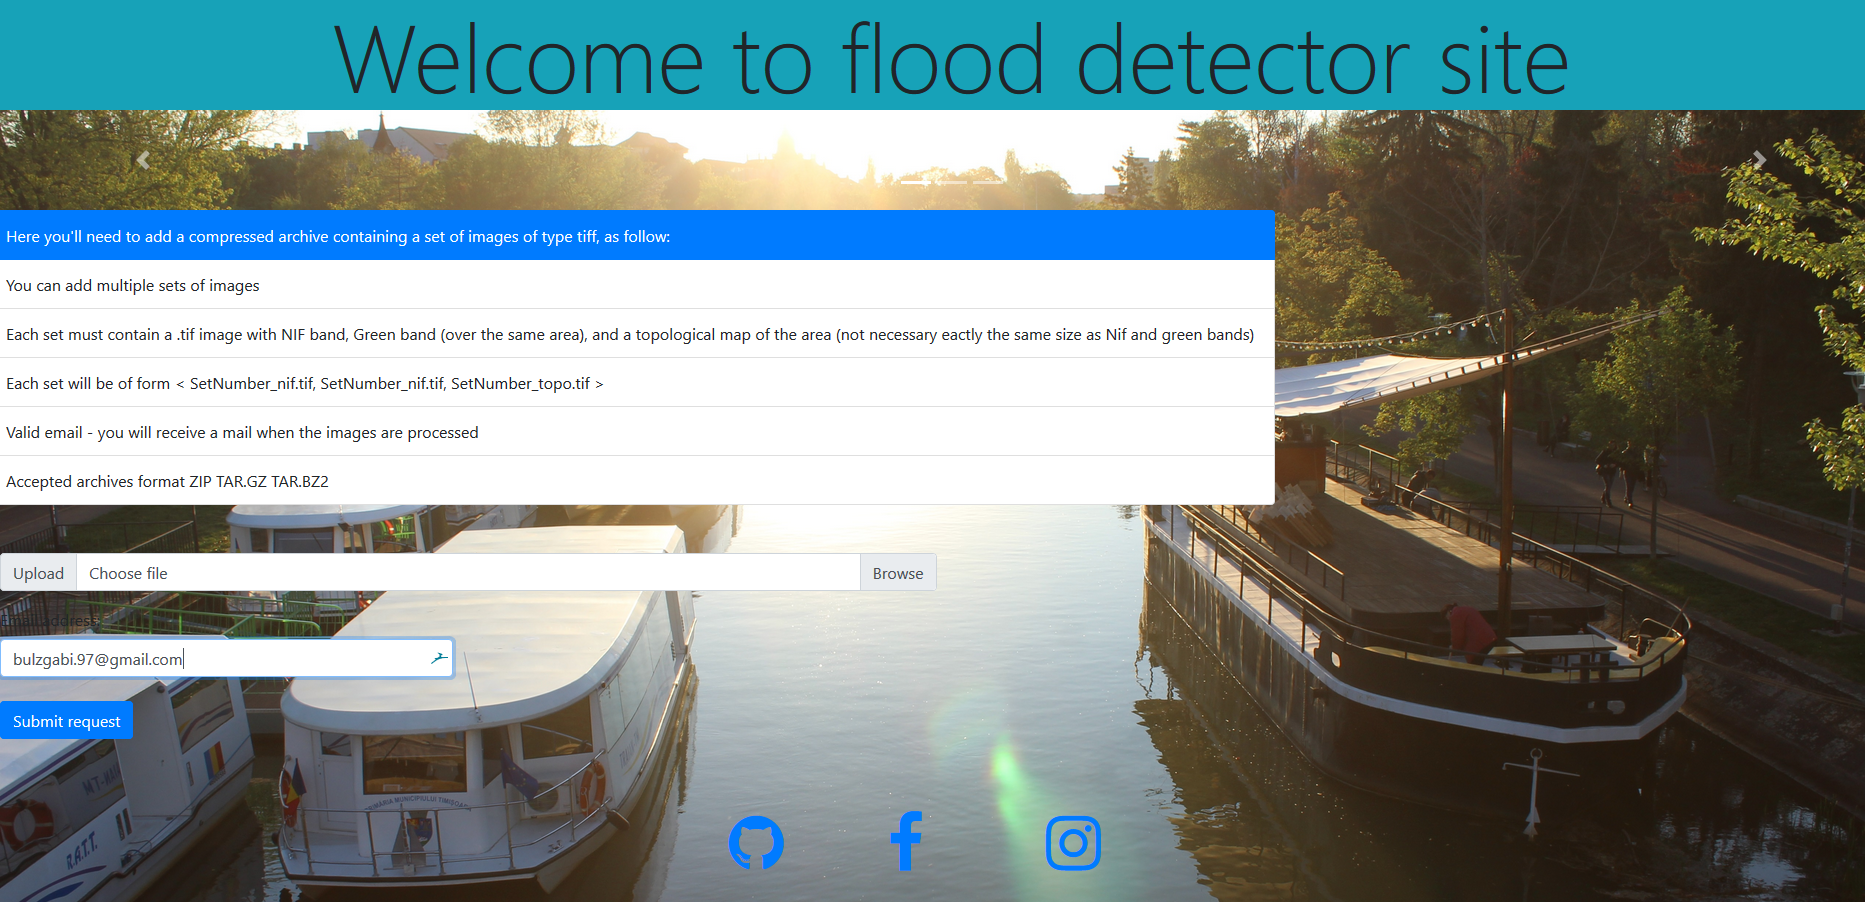
\includegraphics[scale=0.4, center]{gui_homepage.png}
\begin{center}
Figure 18. Main Home Page. 
\end{center}
\par 

The background is a Bootstrap carousel that will display 3 images from our local source, in a repetitive manner. The first item that we see below the title is a Bootstrap list-group that holds several list-group-items, each of them representing an instruction about how the input file should look like (type of accepted images, what images will be needed, accepted naming style, and accepted archives format).
\par 

The second field is a file-input from which the user will be able to upload the archive containing the input images that will later be processed by our server.
\par 

The third field represents an input of type email, where the user should insert an email address to which a message will be sent with a link from where the resulted images can be downloaded, after the server manages to process the request. If an error will occur during the processing the user will be notify at that email address. Below the email input field is a submit button that will upload the images to the server, together with the email address and, if no errors occurred, a web page containing the "Success" message will be displayed. Otherwise a page containing the possible problems will be shown. At the bottom of the page we can find three icons that are linked to our Github, Facebook, and Instagram account.



\section{Main use cases}

\bigskip
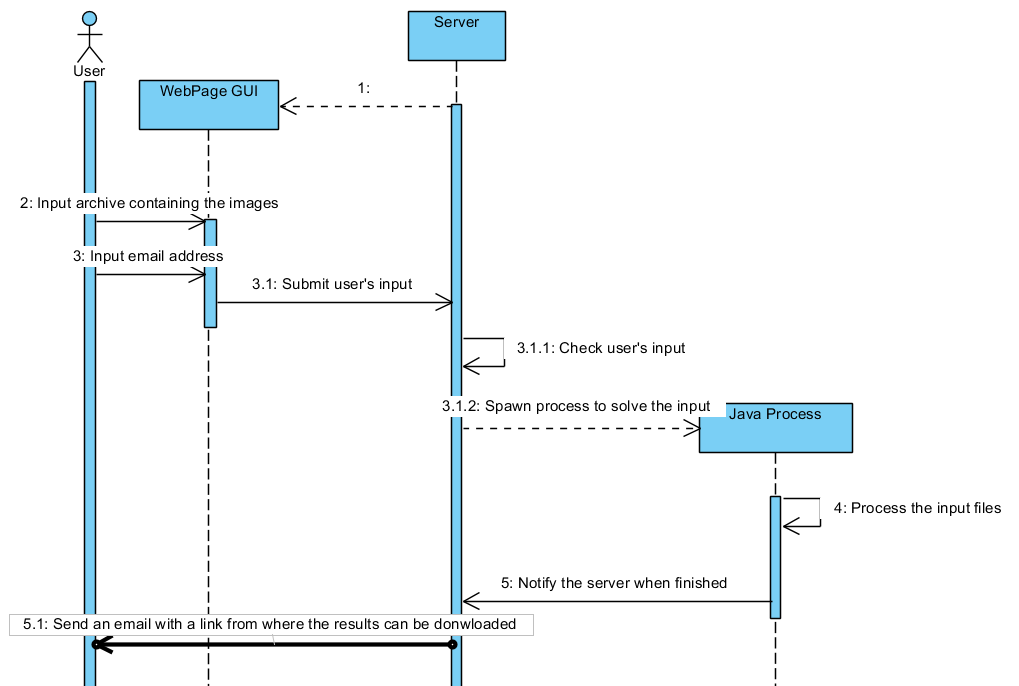
\includegraphics[scale=0.7, center]{FlowCase.png}
\begin{center}
Figure 19. Main use case.
\end{center}
\par 

The figure above (Figure 19) represents the main use case for our application. The flow shows the fact that the Server will deliver a web page for every user, which will input a set of images (archived) and an email back to the page. The user's input will be sent back to the server, and checked for any errors (wrong input images, wrong naming style). If no errors are found the server will spawn a java process that will solve the request and notify the server when the job is completed. If no errors were detected while processing the files, the server will fire an email to the user with a link from where our predictions can be downloaded.


\section{Implementation details}
\quad
In this section we will go a bit deeper in the implementation details of our application. Firstly we will discuss about the server-side written in Python and then we will discuss about the Java part that is responsible for the image processing part.
\par 

In the following picture (Figure 20) we can see an overview of our server, which contains two threads, one is responsible with the web part (with Flask), and the other one is responsible for managing the requests pushed on queue. A Java process is spawned to solve every request and the results path, together with an unique hash, are stored in the database.
\par 

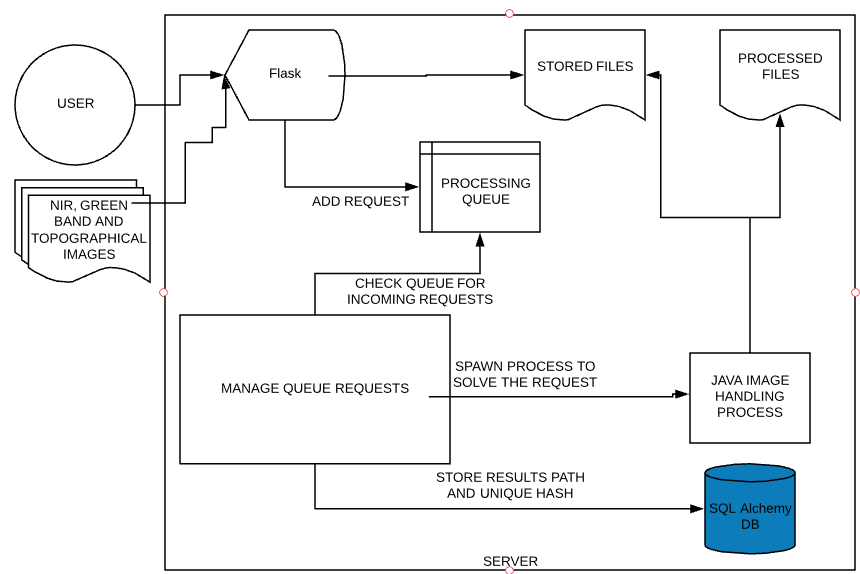
\includegraphics[scale=0.7, right]{application_overview.png}
\begin{center}
Figure 20. Application Structure.
\end{center}
\par 

\subsection{Server Part}

\quad 
The server basically runs on two separate threads that are started when the python process is spawned. One of the threads will be responsible of holding the Flask server, which itself is multi-threaded and can offer multi-user access at the same time. The other thread is responsible for managing the queue where the request are stored.
\par 

When a user submits a request the zipped file is saved in a folder and a processing request containing the user's email address and the path to where the file has been saved, is place into the queue. 
\par 

At first, when the thread responsible for the processing queue is started it compiles all the java classes together with the required libraries (Figure 8). The paths to the java libraries and classes are hardcoded in the python file, and can be changed manually if the location of the java files will ever need to be changed. We do not recommend that thing since all the server components should be stored together to offer a good project structure. All the compiling and spawning of java processes is done using the subprocess library available for python. 
\par 

After the Java files are being compiled the resulted classes are stored into a predefined folder. After that the handling of the queue's requests is started. If the queue is empty then the thread will wait until a request will be placed on the queue. After a request is detected it will be popped from the queue and it will be processed. The input set will be unzipped into a folder with the same name (if it can be created; otherwise it will be renamed), and the content of the that folder will be checked to make sure that the required images with the required naming style are present. If the requirements are not met the server will fire an email to the user that will specify the fact that the received archive was faulty. If the requirements are met a record is inserted in our database.
\par 

The database is created using the SQL ALCHEMY and the resulted table contains one integer column with a unique ID, a string column that will hold the path to the user's file and a string column that will hold a unique hash for every request. We will see later why we used this hash. In the following picture (Figure 21) we can see the table structure.
\par

\medskip
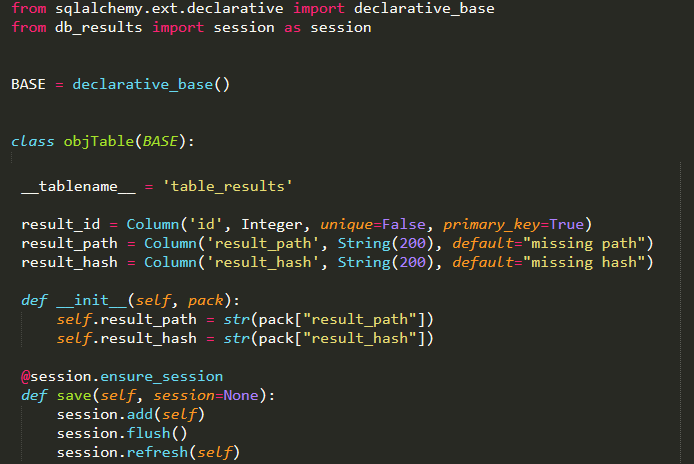
\includegraphics[scale=0.9, right]{database_table.png}
\begin{center}
Figure 21. DB structure created with SQLAlchemy.
\end{center}
\par 

The \textbf{@session.ensure\texttt{\_session}} wrapper is used when an insertion has to occur or an item has to be fetched from the DB. We also provided two functions that can handle this kind of operation \textbf{add\texttt{\_pack}} and \textbf{get\texttt{\_pack}}, which will ensure a new session every time. We created this database as a way to store the information in case of a server failure. If the server will fail we can restore the queue based on this DB or if a result is processed wrong by the java part we can take a look on the faulty files.
\par 

After the server has inserted the information in the database, it will spawn a java process that will handle the images. The java process will place the resulting images into a folder created by the server and when it is done it will return an output to the server that will specify if any error has occurred during the execution. If an error was present the server will fire an email to the user and specify such a situation, otherwise it will send an email containing the link from where the user can download the resulted images. The emails are sent using the smtplib python's library. That library is used to create services that can handle all the emails (@yahoo, @gmail and others).
\par 

The following picture will represent what an user will receive when the server had done processing the request.

\medskip
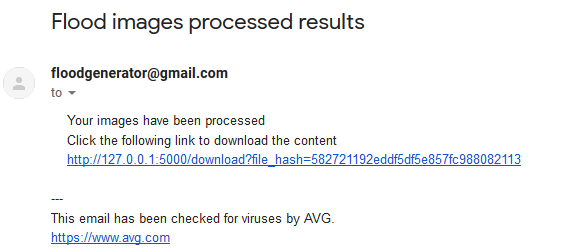
\includegraphics[scale=1, center]{receive_email.png}
\begin{center}
Figure 22. Email received by user containing link to results.
\end{center}
\par 

When the user will click the link a download will be started and, depending on the size, the files will be deleted from the server after a period of time to save storage memory. As we can see in the previous figure (Figure 22) the link contains the file hash stored in our table. If we had chosen to send an email to the user with the file path (default method offered by flask), we would have exposed our server to vulnerabilities, such that if someone would like to download something from our machine it could done that very easily by changing the path. We chose to use a unique hash for every file to prevent this kind of threat.

\subsection{Java part}

\quad 
The first thing that we have to do on our machines to be able to run the server is to slightly modify the Java Virtual Machine (JVM is a virtual machine that enables a machine to run java programs). Because the satellite images that we work with tend to become very large in size we need to allocate some extra memory, such that the java process can load into memory all the files. The images can get as large as 800 Megabytes, and the minimum required number of images for the processing to be done is 3 (NIR, green band and topographical image). A user can upload multiple sets of these kind of images and for every image set a thread will be spawned by the java process, so we will need lots of available memory. On our machine we set up a maximum number of 3 threads that can run simultaneously and we had to set up the default JVM memory to 4 GB. This can be done on a machine running windows by  creating an environment variable called \texttt{\_JAVA\_OPTIONS} with the value \textbf{-Xmx4096m}. That value will set the minimum JVM memory allocation to 4 GB.
\par 

The arguments between the python server and the spawned java process will be passed through the command line. The first argument will be the path to the folder where the images are stored on the server and the second argument will represent the path to where the results should be stored.
\par 

We created two main classes that will handle the images. The first one, which will be instantiated, is named WaterDetectorBasic (Figure 23)and the second one is called CreateFloodMapBasedOnTOPO (Figure 24). The first class (WaterDetectorBasic) contains an inner class called \texttt{Thread\_process\_color}. That will be used as a thread to process every set of images contained in a request. If an input has multiple sets of images a thread will be spawned for each one. Because of our machine's limitation, currently, we are running on maximum 3 threads for each java process (all the images would need to be loaded into memory and we only have 4 GB allocated for the JVM). The threads are spawned using a Java ExecutorService which can create a JavaPool with a predetermined number of threads. A java pool is like a job dispenser with a limited number of employees. You can set the number of employees, each one receiving one task, and when a task is finished by an employee the dispenser will provide another one for it.

\medskip
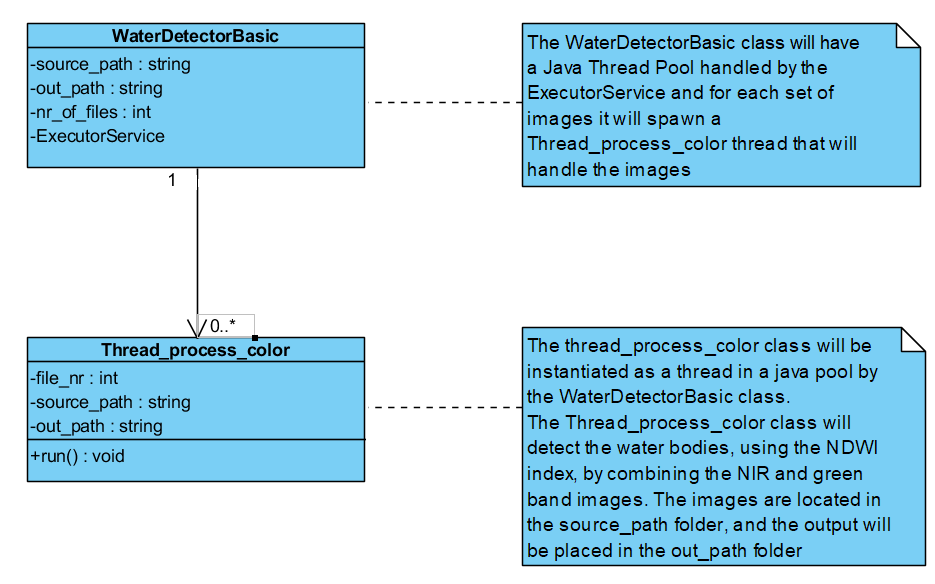
\includegraphics[scale=0.6, center]{WaterDetectorBasic_class.png}
\begin{center}
Figure 23. WaterDetectorBasic class diagram.
\end{center}
\par 

In the above figure (Figure 23) we can see a class diagram representation from WaterDetectorBasic. This class is responsible for detecting the water bodies from the satellite images. For each image set it will spawn a thread that will do the computation using the NDWI index.
\par 

The second important class is called CreateFloodMapBasedOnTOPO and it is pretty similar to our first class. It has a java ExecutorService which creates a java pool that will spawn a thread for every set of images. The thread is an inner class called \texttt{ Thread\_process\_flood }that will create a flood fill based on the land's topography. It has some interesting methods like getPixelFromCoordinates, that can map a certain set of global coordinates to a pixel from an image, and getCoordinatesFromPixel. It also has a method for calculating the distance between 2 given points and a function getHeightFromTopo that will return a value representing the height of a specified coordinates set from a topographical image.

\bigskip
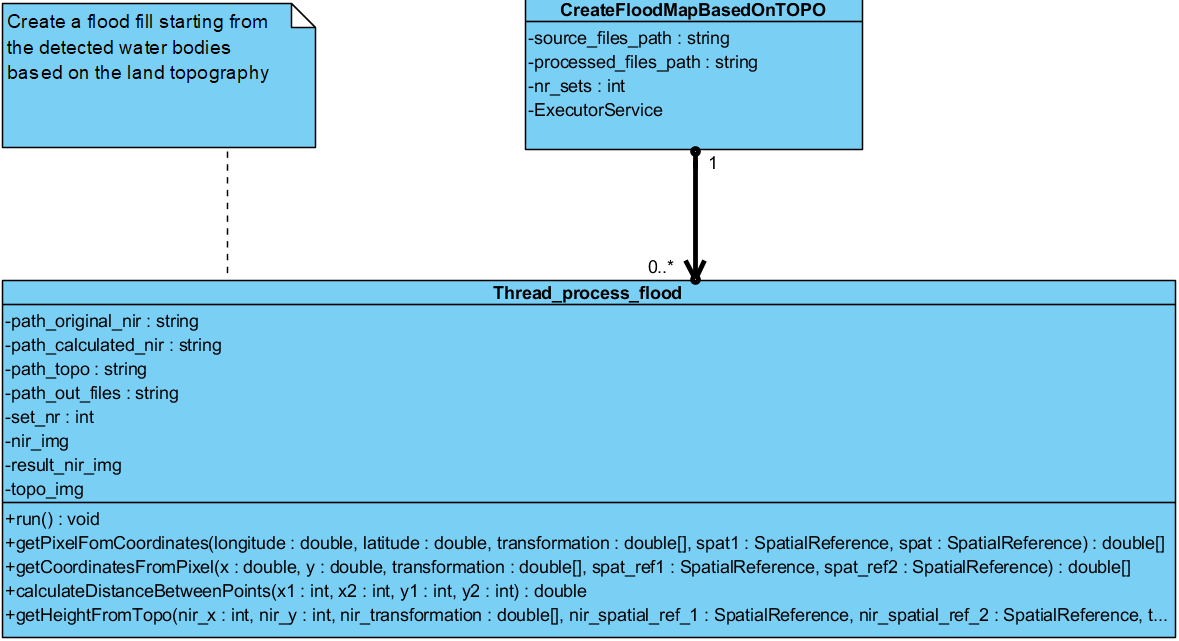
\includegraphics[scale=0.55, center]{CreateFloodMapBasedOnTOPO_class.png}
\begin{center}
Figure 24. CreateFloodMapBasedOnTOPO class diagram.
\end{center}
\par 

\newpage


%\chapter{\vspace{-60pt} Performance Evaluation}
\chapter{Tests}


\bigskip
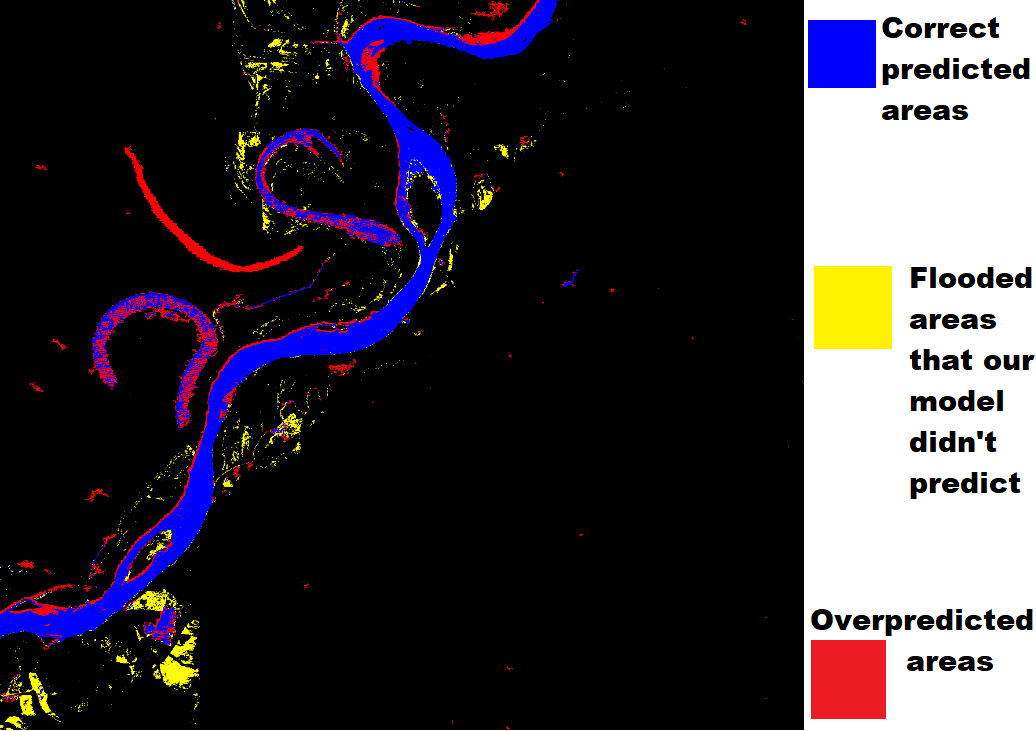
\includegraphics[scale=0.55, center]{test_1_1.png}
\begin{center}
Figure 25. Test 1.
\end{center}
\par 

The test area was located in the Louisiana State, USA, and the comparison was made based on a flood occurred on the Mississipi river on 26.05.2011. The land area covers around \textbf{22,235,760 $m^2$}. The calculated flooded area from 2011 was \textbf{1,129,980 $m^2$} and the area identified correct by our model was \textbf{899,900 $m^2$}, so our prediction had an accuracy of \textbf{79,64\%}. The area that our model was unable to predict was about \textbf{230,080 $m^2$} and the overpredicted area was \textbf{454,830 $m^2$.}

\newpage

\bigskip
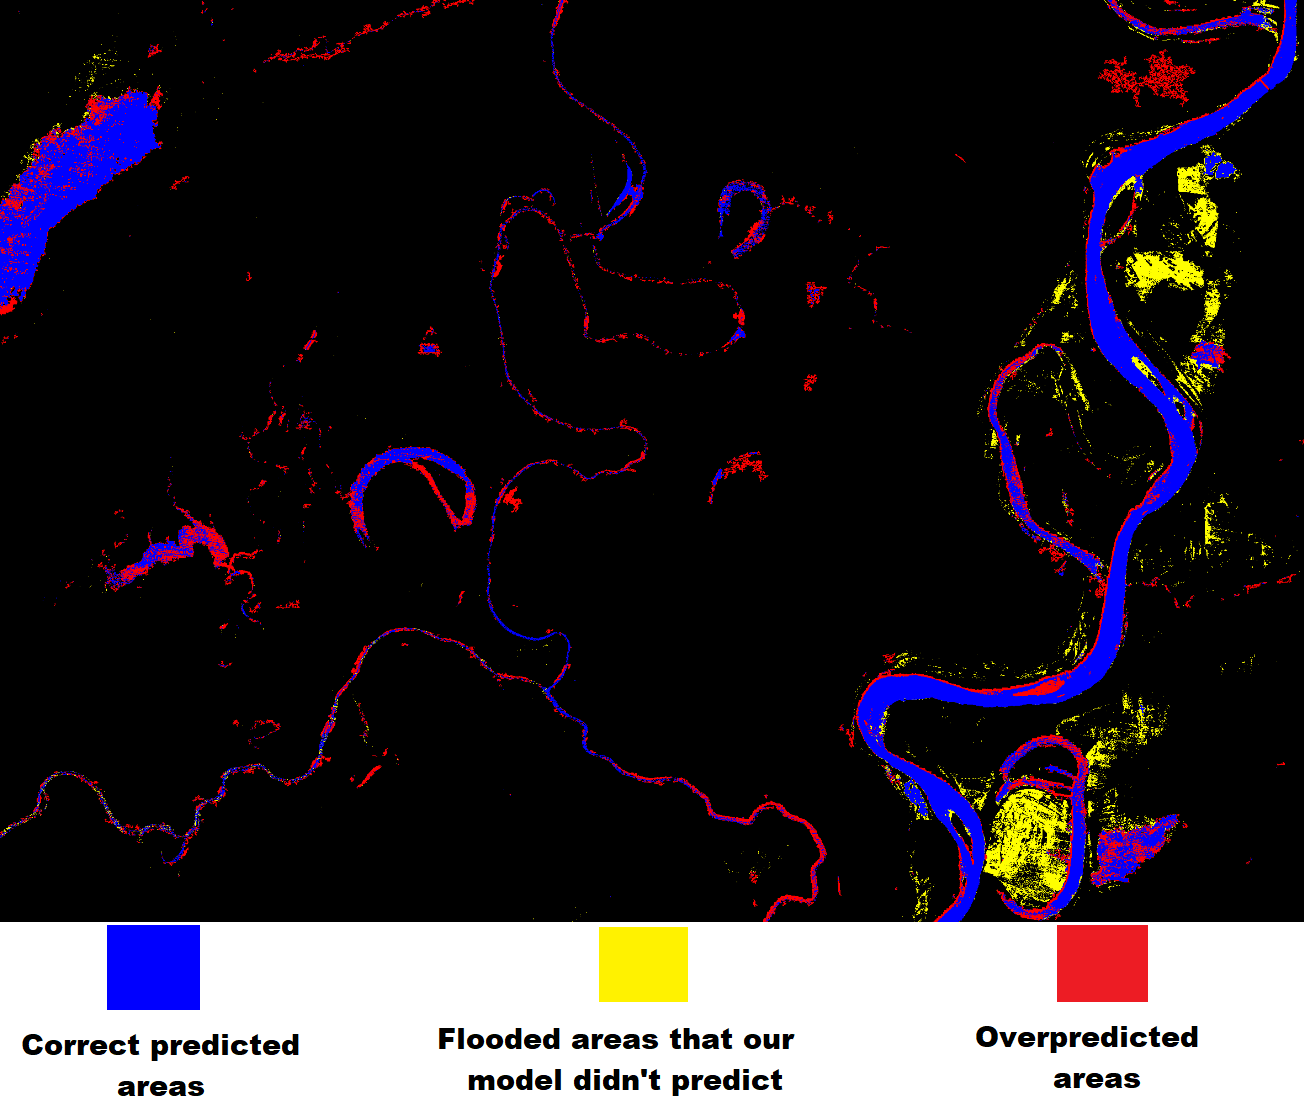
\includegraphics[scale=0.55, center]{test_2.png}
\begin{center}
Figure 26. Test 2.
\end{center}
\par 

The test area was located in the Louisiana State, USA, and the comparison was made based on a flood occurred on the Mississipi river on 26.05.2011. The land area covers around \textbf{42,344,390 $m^2$}. The calculated flooded area from 2011 was \textbf{1,832,910 $m^2$} and the area identified correct by our model was \textbf{1,290,730 $m^2$}, so our prediction had an accuracy of \textbf{70,4\%}. The area that our model was unable to predict was about \textbf{542,180 $m^2$} and the overpredicted area was \textbf{890,335 $m^2$.}

\newpage

\bigskip
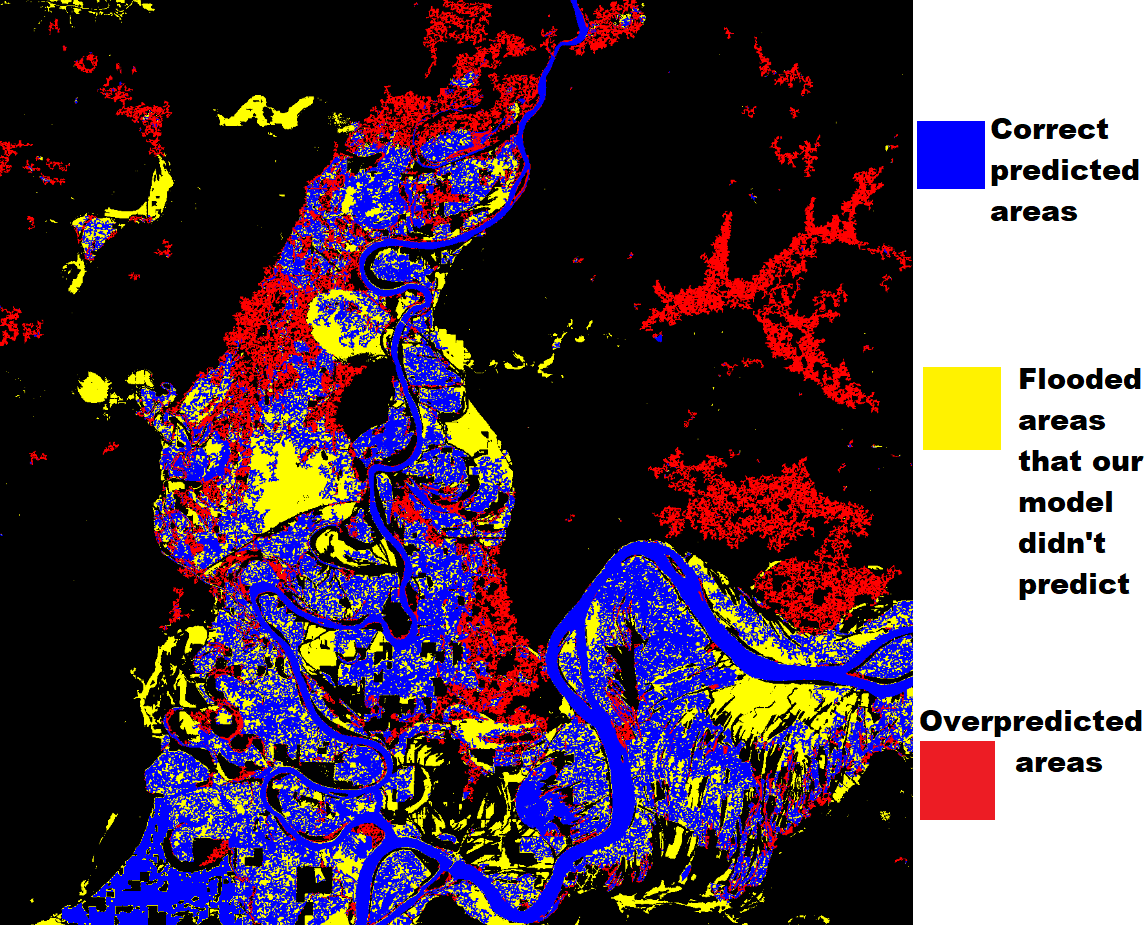
\includegraphics[scale=0.6, center]{test_3.png}
\begin{center}
Figure 27. Test 3.
\end{center}
\par 

The test area was located in the Illinois State, USA, near city of Cairo and the comparison was made based on a flood occurred on the Mississipi river on 11.05.2011. The land area covers around \textbf{20,405,522 $m^2$}. The calculated flooded area from 2011 was \textbf{5,682,310 $m^2$} and the area identified correct by our model was \textbf{3,421,210 $m^2$}, so our prediction had an accuracy of \textbf{60,20\%}. The area that our model was unable to predict was about \textbf{2,261,100 $m^2$} and the overpredicted area was \textbf{1,699,550 $m^2$.}

\newpage

\bigskip
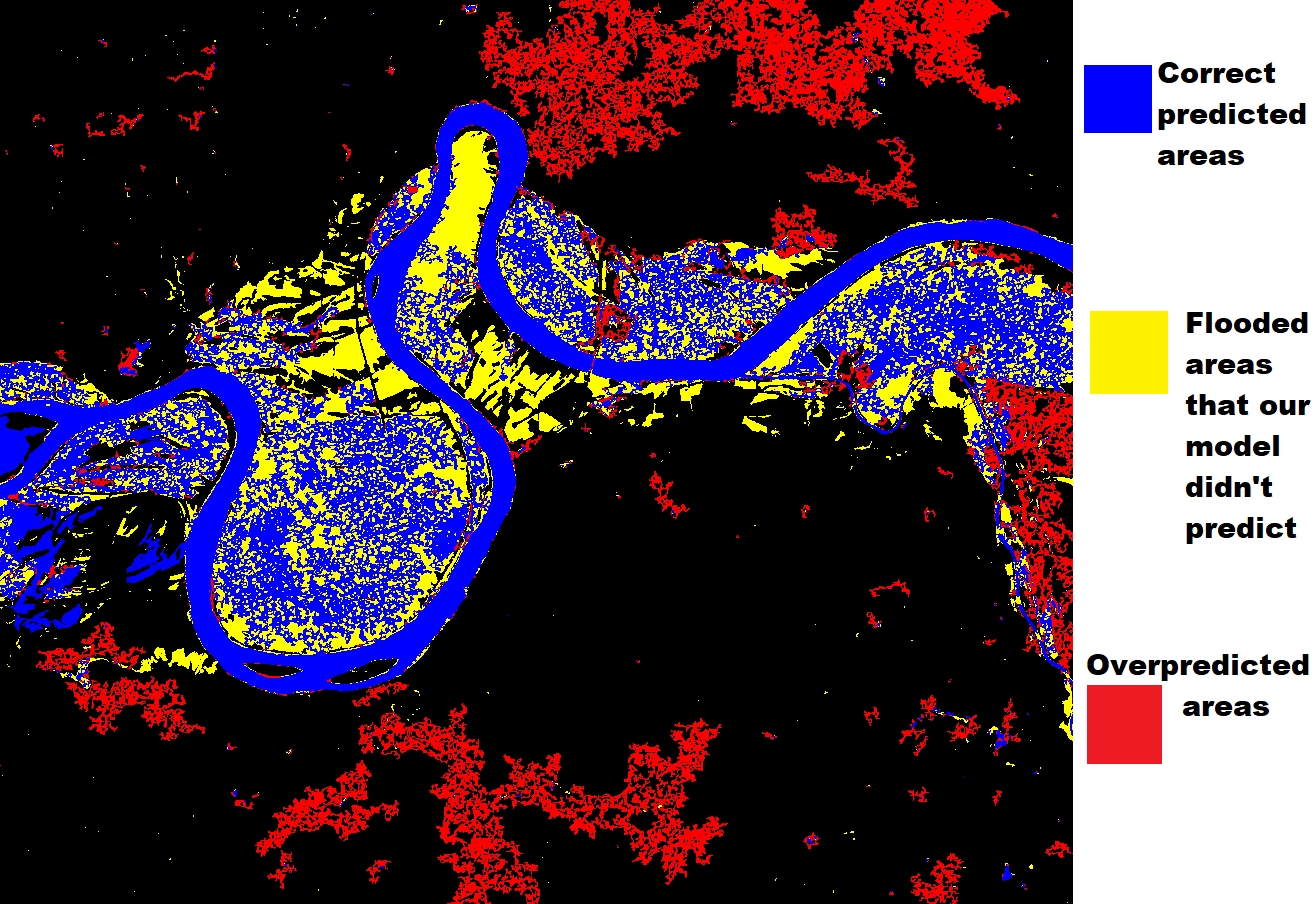
\includegraphics[scale=0.5, center]{test_4.png}
\begin{center}
Figure 28. Test 4.
\end{center}
\par 

The test area was located in the Illinois State, USA, near city of Cairo and the comparison was made based on a flood occurred on the Mississipi river on 11.05.2011. The land area covers around \textbf{9,831,360 $m^2$}. The calculated flooded area from 2011 was \textbf{2,360,730 $m^2$} and the area identified correct by our model was \textbf{1,442,710 $m^2$}, so our prediction had an accuracy of \textbf{61,12\%}. The area that our model was unable to predict was about \textbf{918,020 $m^2$} and the overpredicted area was \textbf{808,500 $m^2$.}

\newpage

\bigskip
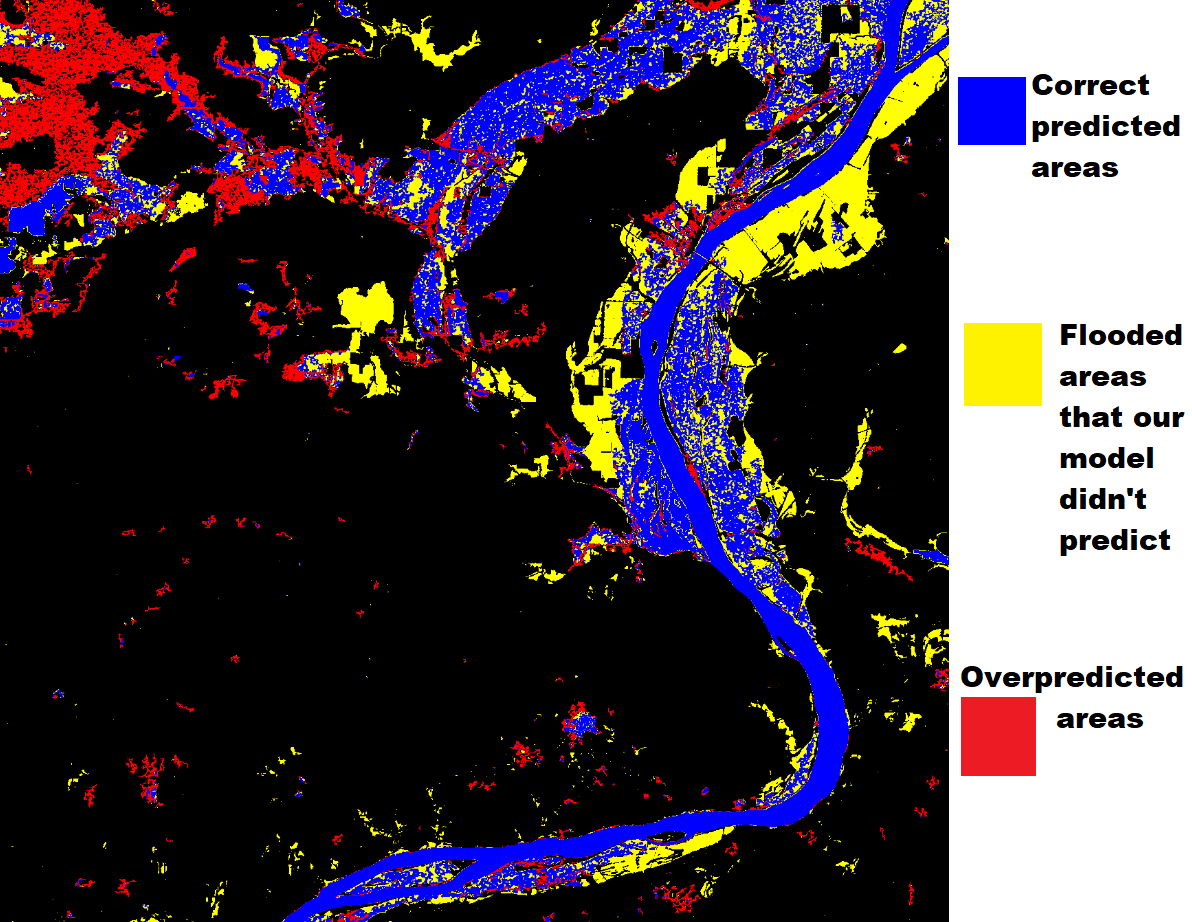
\includegraphics[scale=0.5, center]{test_5.png}
\begin{center}
Figure 29. Test 5.
\end{center}
\par 

The test area was located in the Illinois State, USA, near city of Cairo and the comparison was made based on a flood occurred on the Mississipi river on 11.05.2011. The land area covers around \textbf{18,738,000 $m^2$}. The calculated flooded area from 2011 was \textbf{3,576,710 $m^2$} and the area identified correct by our model was \textbf{2,067,510 $m^2$}, so our prediction had an accuracy of \textbf{57.80\%}. The area that our model was unable to predict was about \textbf{1,509,200 $m^2$} and the overpredicted area was \textbf{855,590 $m^2$.}

\newpage

\bigskip
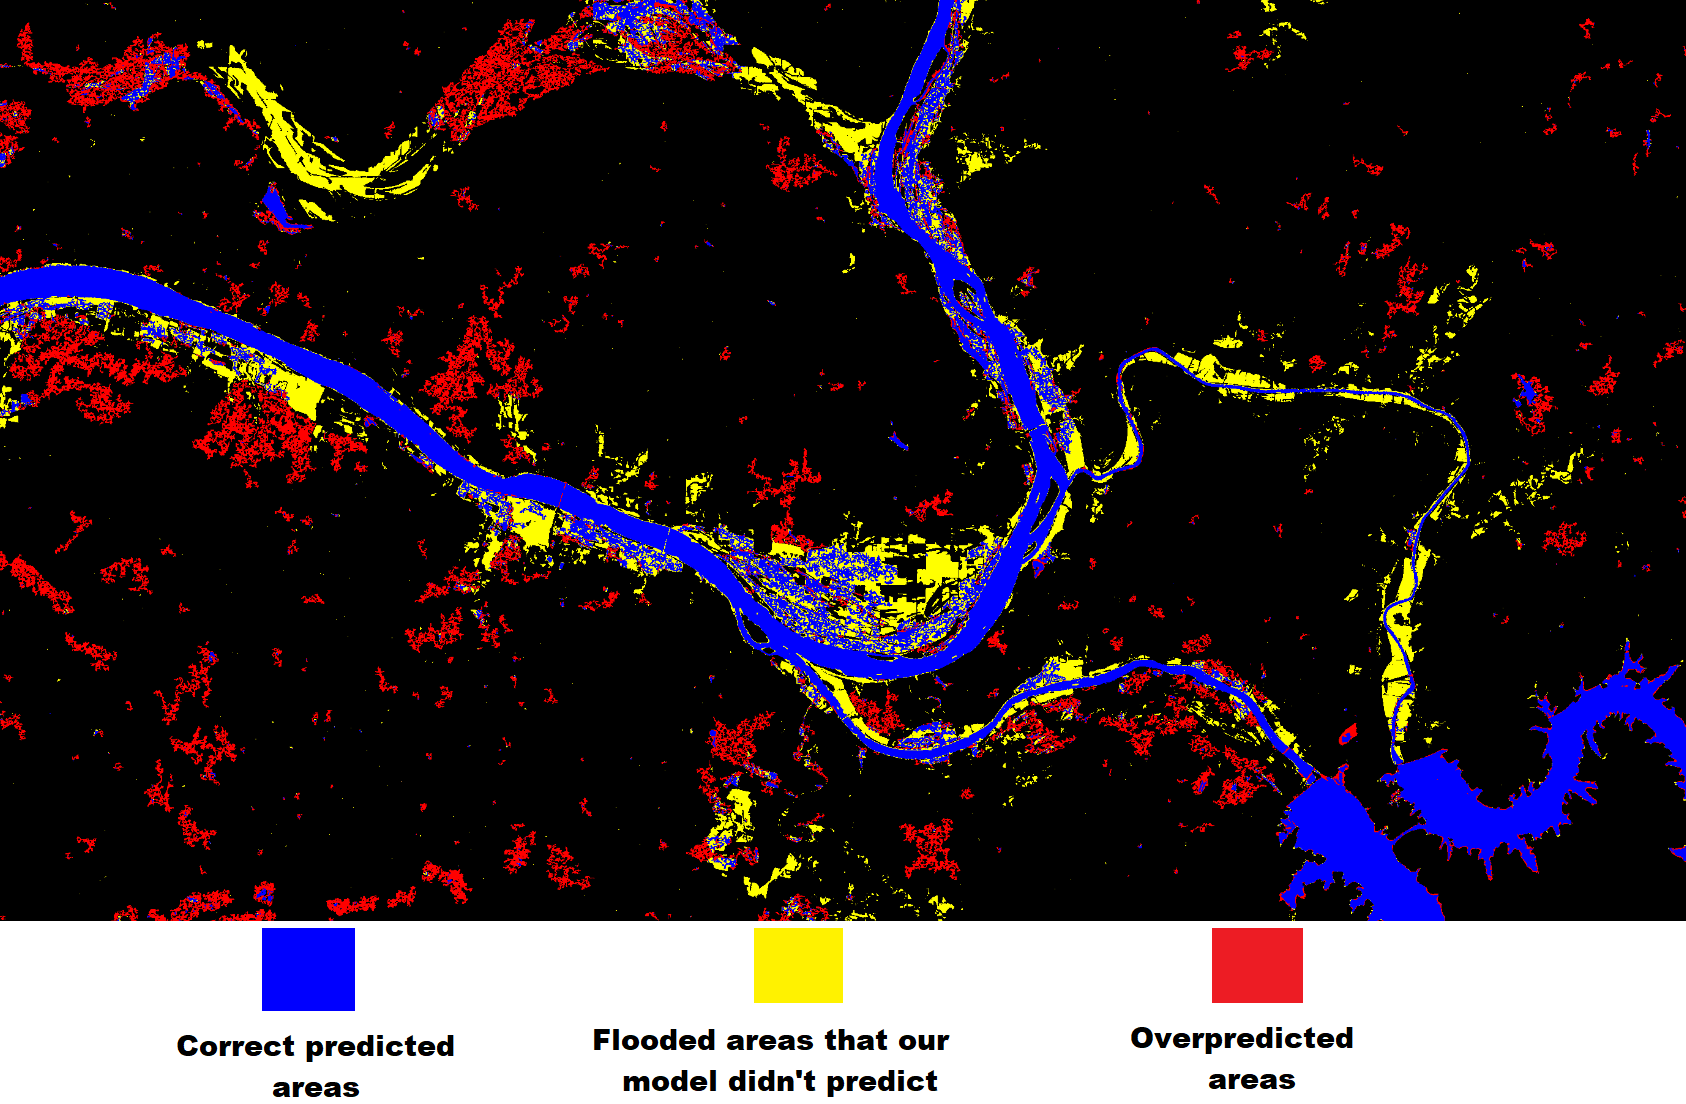
\includegraphics[scale=0.4, center]{test_6.png}
\begin{center}
Figure 30. Test 6.
\end{center}
\par 

The test area was located in the Illinois State, USA, near city of Cairo and the comparison was made based on a flood occurred on the Mississipi river on 11.05.2011. The land area covers around \textbf{42,129,640 $m^2$}. The calculated flooded area from 2011 was \textbf{4,551,300 $m^2$} and the area identified correct by our model was \textbf{2,907,040 $m^2$}, so our prediction had an accuracy of \textbf{63,87\%}. The area that our model was unable to predict was about \textbf{1,644,260 $m^2$} and the overpredicted area was \textbf{1,224,370 $m^2$.}

\newpage

\bigskip
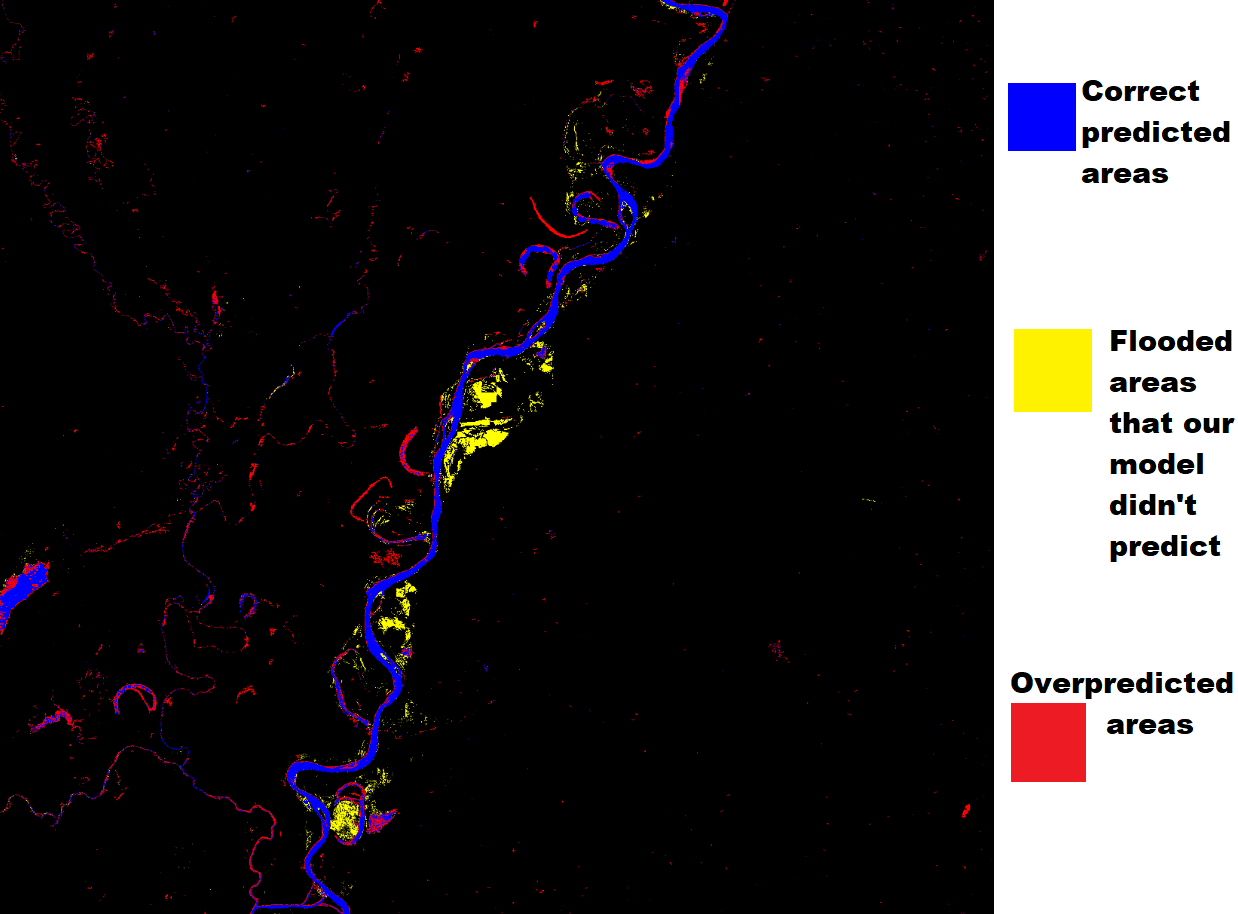
\includegraphics[scale=0.5, center]{test_7.png}
\begin{center}
Figure 31. Test 7.
\end{center}
\par 

The test area was located in the Louisiana State, USA, and the comparison was made based on a flood occurred on the Mississipi river on 26.05.2011. The land area covers around \textbf{264,620,250 $m^2$}. The calculated flooded area from 2011 was \textbf{4,688,740 $m^2$} and the area identified correct by our model was \textbf{3,813,420 $m^2$}, so our prediction had an accuracy of \textbf{81,33\%}. The area that our model was unable to predict was about \textbf{875,320 $m^2$} and the overpredicted area was \textbf{2,172,160 $m^2$.}



\clearpage

\chapter{Conclusions and future development}

\section{Future Development}

\quad
One of the first things that we will like to do in the future is to \textbf{transform our physical prediction model into a hybrid prediction model}.
%, that will combine the advantages of the ML models together with the upsides of the physical model.
\par 

We would like to keep, as much as possible, the focus on our goal, by creating an easy to use and cheap to run prediction model that would be available for everyone, with a higher accuracy rate. By tilting to a hybrid model we hope to increase our prediction accuracy from about 67\% to as much as possible, without losing our integrity regarding the application's simplicity and reduced cost.
\par

We could try to add new factors in our model that would dramatically increase the accuracy, like \textbf{taking into account the actual precipitation volume} over a land area and the \textbf{water flow over some regions}. Taking into account these factors will surely increase the development and running cost, because the model will be much more complex and will require more processing time. Another factor that could increase our accuracy rate, that will be rather cheap and easy to integrate, would be to \textbf{analyze the plants and the soil}. That could be done pretty easily, by adding one more photo to the data set (from the user's point of view), and by combining the pictures we could determine the water level from the soil and the type of plans that grow over a land area. The plants can have a big impact because they can absorb huge quantities of water and they can also change the water's path during a flood.
\par 
All these factors can surely increase our prediction model accuracy rate, but we will need to keep in mind our goal, to create an easy to use and cheap prediction model.

\newpage


\section{Conclusions}

\quad 
In conclusion we can say that we are satisfied with the obtained results because we had a main goal in mind when we started this project. The main plan was to create an easy to use and cheap to create and run program that can offer considerable results on detecting the areas with a high risk of being flooded during a heavy rainstorm.
\par 

The water identification part, using the NDWI index, showed remarkable detection accuracy, of around \textbf{89\%} (from our tests), without making many false positive assumptions. The water zones that our model may fail to identify are the water regions that are not too deep, like the river banks and small ponds, but usually these don't have huge impact during a flood when we take into consideration the water volume that will be delivered by lakes and rivers.
\par 

The prediction of areas with high risk of being flooded had an accuracy rate of around \textbf{67\%} (from our tests that compared the predicted areas with the flooded areas from previous incidents), and from our point of view the model could offer some valuable information. For example, our system could be used by normal people to identify the places where it could be safe to build a house or invest in agriculture.




\renewcommand{\bibname}{Bibliography}

\bibliographystyle{Plain} % Plain, Abbrv, Unsrt, Alpha
\addcontentsline{toc}{chapter}{Bibliography} 

\begin{thebibliography} {10}

%\begin{thebibliography}{widest entry}
\bibitem{Rover} Rover J., Ji L., Wylie B.K., Tieszen L.L. Establishing Water Body Areal Extent Trends in Interior Alaska from Multi-Temporal Landsat Data. Remote Sens. Lett. 2012;3:595–604. doi: 10.1080/01431161.2011.643507

\bibitem{Alsdorf} Alsdorf D.E., Rodríguez E., Lettenmaier D.P. Measuring Surface Water from Space. Rev. Geophys. 2007;45 doi: 10.1029/2006RG000197. [CrossRef] [Google Scholar]

\bibitem{Flood-forecasting}
Flood forecasting - World meteorological organization \textit{http://www.wmo.int/pages/prog/hwrp/FloodForecastingInitiative.php} - accessed in 15.05.2019


\bibitem{Xie} Xie, K; Ozbay,K;Zhu, Y;Yang, H. Evacuation zone modeling under climate change: A data-driven method. J.Infrastruct. Syst. 2017,23,04017013

\bibitem{Pitt}Pitt, M.	Learning Lessons from the 2007 Floods; Cabinet Office: London, UK, 2008.

\bibitem{Lohani}Lohani, A.K.; Goel, N.; Bhatia, K. Improving real time flood forecasting using fuzzy inference system.J. Hydrol. 2014, 509, 25–41

\bibitem{Nayak}Nayak, P.; Sudheer, K.; Rangan, D.; Ramasastri, K. Short-term flood forecasting with a neurofuzzy model.Water Resour. Res. 2005, 41.

\bibitem{Taherei}Taherei Ghazvinei, P.; Hassanpour Darvishi, H.; Mosavi, A.; Yusof, K.B.W.; Alizamir, M.; Shamshirband, S.; Chau, K.W. Sugarcane growth prediction based on meteorological parameters using extreme learning machine and artificial neural network. Eng. Appl. Comput. Fluid Mech. 2018, 12, 738–749

\bibitem{Kasiviswanathan}Kasiviswanathan, K.; He, J.; Sudheer, K.; Tay, J.-H. Potential application of wavelet neural network ensemble to forecast streamflow for flood management. J. Hydrol. 2016, 536, 161–173.

\bibitem{Ravansalar}Ravansalar, M.; Rajaee, T.; Kisi, O. Wavelet-linear genetic programming: A new approach for modeling monthly streamflow. J. Hydrol. 2017, 549, 461–475.

\bibitem{Mosavi}Mosavi, A.; Rabczuk, T. Learning and intelligent optimization for material design innovation. In Learning and Intelligent Optimization; Springer: Cham, Switzerland, 2017; pp. 358–363.

\bibitem{Dandagala}Dandagala, S.; Reddy, M.S.; Murthy, D.S.; Nagaraj, G. Artificial neural networks applications in groundwater hydrology—A review. Artif. Intell. Syst. Mach. Learn. 2017, 9, 182–187.

\bibitem{Deka}Deka, P.C. Support vector machine applications in the field of hydrology: A review. Appl. Soft Comput. 2014,
19, 372–386.

\bibitem{Fotovatikhah}Fotovatikhah, F.; Herrera, M.; Shamshirband, S.; Chau, K.-W.; Faizollahzadeh Ardabili, S.; Piran, M.J. Survey of computational intelligence as basis to big flood management: Challenges, research directions and future work. Eng. Appl. Comput. Fluid Mech. 2018, 12, 411–437. 

\bibitem{McFeeters}McFeeters, S.K. The use of the normalized difference water index (NDWI) in the delineation of open water features. Int. J. Remote Sens. 1996, 17, 1425–1432.

\bibitem{Duan}Duan, Z.; Bastiaanssen, W.G.M. Estimating water volume variations in lakes and reservoirs from four operational satellite altimetry databases and satellite imagery data. Remote Sens. Environ. 2013, 134, 403–416.

\bibitem{Poulin}Poulin, B.; Davranche, A.; Lefebvre, G. Ecological assessment of phragmites australis wetlands using multi-season spot-5 scenes. Remote Sens. Environ. 2010, 114, 1602–1609..

\bibitem{Hui}Hui, F.; Xu, B.; Huang, H.; Yu, Q.; Gong, P. Modelling spatial-temporal change of poyang lake using multitemporal landsat imagery. Int. J. Remote Sens. 2008, 29, 5767–5784.

\bibitem{Multifractal water analysis}
Multifractal Analysis of Hydrologic Data -
Tongzhou Zhao, Liang Wu, Dehua Li, Yiming Ding, Multifractal Analysis of Hydrologic Data Using Wavelet Methods and Fluctuation Analysis, published in Discrete Dynamics in Nature and Society
Volume 2017

\bibitem{NDWI Comparison}
Comparison between NDWI, Machine Learning, and Multifractal analysis for detecting water bodies -  
V. M. San Martina, Alejandra Figliolaa, Application of Multifractal Analysis to Segmentation of WaterBodies in Optical and Synthetic Aperture Radar Satellite Images, originally announced April 2016 and published in Cornell University Journal.

\bibitem{Flood forecasting models}
Flood forecasting models - S. Nevo, V. Anisimov, G. Elidan, R. El-Yaniv, P. Giencke, Y. Gigi, A. Hassidim, Z. Moshe, M. Schlesinger, G. Shalev, A. Tirumali, A. Wiesel, O. Zlydenko, Y. Matias ,  ML for Flood Forecasting at Scale originally announced in January 2019, published in 28 January 2019 on arXiv.

\bibitem{Yohai}
ML hydro-dynamic modeling
Yohai Bar-Sinai, Stephan Hoyer, Jason Hickey, and Michael P Brenner. Data-driven discretiza-tion: a method for systematic coarse graining of partial differential equations.arXiv preprintarXiv:1808.04930, 2018


\bibitem{USGS}
USGS \textit{https://earthexplorer.usgs.gov/} - accessed in 19.05.2019


\bibitem{Wiki_landsat}
Wikipedia Landsat Program \textit{https://en.wikipedia.org/wiki/Landsat\_program} - accessed in 19.05.2019

\bibitem{Copernicus}
Copernicus \textit{https://scihub.copernicus.eu/} - accessed in 19.05.2019

\bibitem{QGIS}
QGIS \textit{https://www.qgis.org/en/site/about/index.html} - accessed in 19.05.2019

\bibitem{Landsat-error}
Landsat-error \textit{https://www.pixalytics.com/landsat-quirks/} - accessed in 22.05.2019

\bibitem{Gdal}
Gdal \textit{https://en.wikipedia.org/wiki/GDAL} -accessed in 22.05.2019

\bibitem{Flask1}
Flask vs Django \textit{http://www.mindfiresolutions.com/blog/2018/05/flask-vs-django/} -accessed in 22.05.2019

\bibitem{Flask2}
Flask server vs Django server \textit{http://blog.gmludo.eu/2015/02/macro-benchmark-with-django-flask-and-asyncio.html} -accessed in 22.05.2019

\bibitem{NDWI}
A. S. Rogers, M. S. Kearney, Reducing signature variability in unmixing coastal marshthematic mapper scenes using spectral indices, International Journal of Remote Sensing25 (12) (2004) 2317–2335.






\end{thebibliography}






% end appendix part

\end{document}
